                                  \documentclass[11pt, twocolumn]{report}
\usepackage[a4paper, hmargin={2.8cm, 2.8cm}, vmargin={2.5cm, 2.5cm}]{geometry}
%\usepackage[T1]{fontenc}
\usepackage[utf8]{inputenc}
\usepackage{eso-pic} % \AddToShipoutPicture
\usepackage{graphicx} % \includegraphics
\usepackage[english]{babel}
\usepackage{tcolorbox}
\usepackage{multicol}
\usepackage{amssymb}
\usepackage{amsmath}
\usepackage{fancyhdr}
\usepackage{fancyvrb}
\usepackage{geometry}
\usepackage{listings}
\usepackage[hyphens]{url}
\usepackage{breakurl}
\usepackage{cite}
\usepackage{color}
\usepackage{array}
\usepackage{multicol}
\usepackage{subcaption}
\usepackage[toc,page]{appendix}
\usepackage[breaklinks=true]{hyperref}
\usepackage{float}
\usepackage{xcolor}
\usepackage{tablefootnote}
\usepackage{footnote}
\usepackage{lipsum}
\usepackage{tocloft}
\usepackage{blindtext}
\usepackage{enumitem}
\usepackage{minted}

\usepackage{coffee4} % Comment me out


% Define Listings
\definecolor{codegreen}{rgb}{0,0.6,0}
\definecolor{codegray}{rgb}{0.5,0.5,0.5}
\definecolor{codepurple}{rgb}{0.58,0,0.82}
\definecolor{codeblue}{rgb}{0,0,0.95}
\definecolor{backcolour}{rgb}{0.95,0.95,0.95}

\lstdefinestyle{sme}{
    backgroundcolor=\color{backcolour},
    commentstyle=\color{codegreen},
    keywordstyle=\color{codeblue},
    numberstyle=\tiny\color{codegray},
    stringstyle=\color{codeblue},
    basicstyle=\ttfamily\footnotesize,
    xleftmargin=15pt,
    framexleftmargin=15pt,
    framexrightmargin=2pt,
    framexbottommargin=2pt,
    frame=single,
    breakatwhitespace=false,
    breaklines=true,
    breakatwhitespace=true, % Do not break at "other" characters
    captionpos=b,
    keepspaces=true,
    numbers=left,
    numbersep=5pt,
    showspaces=false,
    showstringspaces=false,
    showtabs=false,
    tabsize=2,
}

\lstset{style=sme}


%%% Macros
% easier figure
% usage: \pic{width}{image}{caption}{label}
\newcommand\pic[4]{% these comment signs will prevent the introduction of spurious spaces
  \begin{figure}[h!]
  \centering
  \includegraphics[width=#1\textwidth]{#2}
  \caption{#3}
  \label{#4}
  \end{figure}
}




\newcolumntype{C}[1]{>{\centering\let\newline\\\arraybackslash\hspace{0pt}}m{#1}}
\setlength{\columnsep}{1cm}


\author{
  Meznik, Jan\\
  \texttt{pzj895@alumni.ku.dk}\\
  \texttt{jan@meznik.dk}
  \and
  Jacobi, Mark Jan\\
  \texttt{dcz738@alumni.ku.dk}
}

\title{
	\vspace{3cm}
	\huge{TCP/IP in hardware using SME}\\
		\vspace{0.5cm}
	\Large{Write something clever here}
}



% Header
\pagestyle{fancy}


\iffalse
\fancyhf{}
%\fancyhead[L]{}
%\fancyhead[R]{}
%\fancyhead[C]{}
%\fancyfoot[C]{Center \leftmark}
\fi

\lhead{University of Copenhagen}
%\chead{}
\rhead{TCP/IP in SME}


\begin{document}
\onecolumn


%%%%% KU HEADER %%%%%%%%%%%%%%%%%%%%%%%
\AddToShipoutPicture*{\put(0,0){\includegraphics*[viewport=0 0 700 600]{include/natbio-farve}}}
\AddToShipoutPicture*{\put(0,602){\includegraphics*[viewport=0 600 700 1600]{include/natbio-farve}}}
\AddToShipoutPicture*{\put(0,0){\includegraphics*{include/nat-en}}}
\clearpage
\maketitle
\pagenumbering{roman}
\thispagestyle{empty}
\newpage
%%%%%%%%%%%%%%%%%%%%%%%%%%%%%%%%%%%%%%%


%\begin{abstract}
\thispagestyle{empty}
%In this thesis, we design and implement a networking protocol using the
Synchronous Message Exchange model -- a new framework intended to help model
hardware descriptions.
The final pipelined design boasts with a decentralized memory model, with model
division easily extensible and modifiable, closely ressembling that of the
architecture of the Internet Protocol Suite.

Initial tests performed on the simulated system with real captured network
traffic suggests stability, promising protocol compliance, and an acceptable, but
theoretical, performance. Numerous suggestions are discussed to improve the performance,
such as widening the bus-widths or replicating the stack itself to multiply the
raw throughput.

Due to some trivial bugs and other minor missing features in the SME framework,
the system could not be brought to the target FPGA hardware. However, we are
optimistic that considerable performance is achieveable with the current design,
as well as great flexibility, extensibility and modularity of the system.



\newpage
%\end{abstract}


%\section*{Overview}
%\input{overview/overview.tex}

\newpage

% \section*{Preface}
% \input{preface/preface.tex}
\newpage
\twocolumn

\thispagestyle{empty}
\setcounter{tocdepth}{3} % Add subsubsections to ToC
\tableofcontents
\renewcommand{\cftchapleader}{\cftdotfill{\cftdotsep}}
\renewcommand{\cftsecleader}{\cftdotfill{\cftdotsep}}
\onecolumn
\newpage
\twocolumn

\clearpage
\pagenumbering{arabic}
\setcounter{page}{1}

\markboth{Name}{Report}
\noindent

% Chapters:
\chapter{Introduction}
% 1. general introduction
This thesis describes the design and implementation of an efficient, high-speed
TCP/IP network stack intended to run on custom hardware where performance, responsiveness,
and throughput is crucial.\\

% 2. Explanation of specific problem
As is the trend with modern automation, computerization, and mechanization, new
devices are steadily invented to handle this increasing demand for data and
control.
With the ever-increasing sophistication of machines generating immense amount
of information, the data needs to be transmitted to numerous other machines for
further processing, or even simply storage. The most common and the most convenient
way of linking multiple devices together is using the internet, and its underlying
protocols. However, the networking stack supplied with most major operating
systems, while heavily optimised, suffers from considerable penalties due to
complexities of a standard computer architecture. For example, heavy network
traffic utilizes the computers' internal busses, utilizes the memory, and spend
precious CPU clock-cycles with polling and interrupts. This
prevents the machine from using these resources for actual computing tasks.\\
These issues have been identified and solved by hardware manufacturers by
adopting dedicated Network Interface Controllers (NIC), which would employ
various techniques to offload the processing. One such offloading technique is
called the TCP offload engine (TOE), which usually takes care of the essential
parts of networking involved -- the Internet Protocol (IP) and the Transmission
Control Protocol (TCP) \cite{TCP_offload_dumb_idea}.\\
Modern hardware manufacturers can produce NICs boasting network throughput
speeds as high as 100 Gigabits\cite{xilinx_100g_nic}. Unfortunately, these cards
are highly specialized for certain applications, and even though they provide
basic programmability, they are rarely suitable for rapid prototyping of
applications and other custom hardware devices. Furthermore, each NIC manufacturer
has a diverse set of hardware with varying interfaces, making it hard to
combine, swap and test these cards.
Licensed software solutions in the form of IP blocks exist as well
\cite{microtronix_ip_cores}\cite{avnet_ip_cores}. Unfortunately,
these blocks are usually distributed as black-boxes of VHDL code, which is
hard to maintain, and even harder to debug and extend\cite{opencores_mission}.\\

In this thesis, we bridge the gap between the blazingly-fast network offloading
devices and their more flexible and malleable software counterparts.\\
This networking stack is implemented in a fully self-contained fashion so that
it is completely independent of any other software running on the machine, while
utilizing the performance advantages gained from the lack of overhead in
conventional implementations.
The use of a high-level programming language in combination with the modern
Synchronous Message Exchange (SME) model makes the network stack a very versatile
implementation with ease of use, debugging, and even extension.

% * VHDL unmaintainable
% * SME better for simulation
% * IP blocks not open source (No code) + Hard to debug
% * Price



MORE TO COME!!


% 3. Brief review of existing solutions

% 4. Output of proposed solution

% 5. Summary

\section{Introduction}
\begin{frame}
  \frametitle{Background and Motivation}

FPGAs are making their way into data centers to boost the computing power
	and the overall power efficiency.


\begin{columns}
\begin{column}{0.8\textwidth}
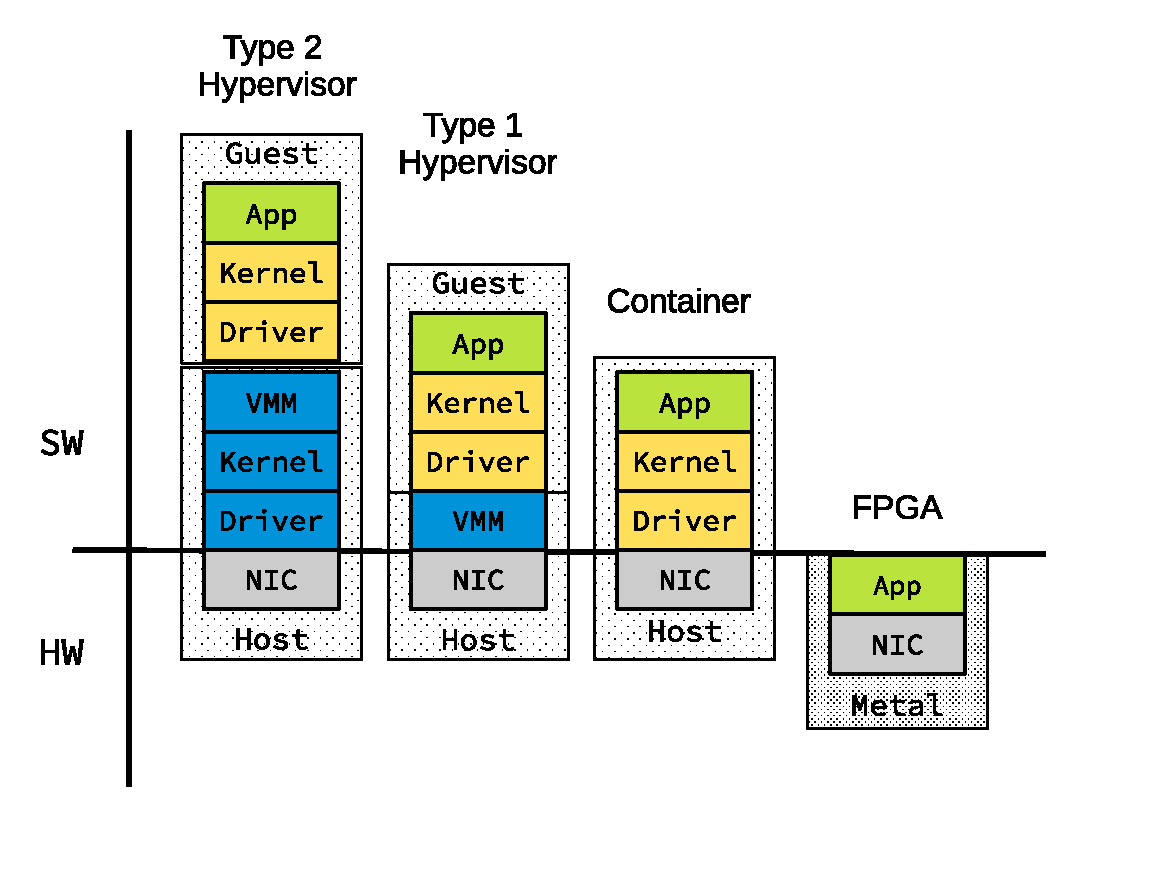
\includegraphics[scale=0.5]{./background/server_configuration.eps}
\end{column}

\begin{column}{0.2\textwidth}
\includegraphics[scale=0.2]{./background/intel_fpga_nic.jpg}
\end{column}
\end{columns}

\end{frame}




\note{Applikationer og Big-Data udregninger flytter til Cloud, drevet af store
data centre.\\

Disse data-centre kraever rigtigt meget plads, store maengder af stroem og er i stigende grad svaere
at vedligeholde og udvide.\\

De fleste data-centre er derfor begyndt at aflaste beregningerne til FPGAer,
som fjerner meget af overhead til beregningerne\\

kan bruges til at få en computer til at køre hurtigere hvis de mest brugte
instruktioner, skrives direkte ned i hardwaren\\

PROBLEMET er at der kun kan vaere en begreanset antal af FPGAer i konventionele
servere

}



% Talking points:


% > In the current era of big data, computationally heavy applications are
% moving to the cloud. ... Consuming wast amount of energy and are increasingly
% complex to maintain and improve

% > To combat this, DC servers offload the computation onto FPGAs

% <SHOW GRAPH HERE>

% > However, this is not scalable in the conventional DC architecture, as the
% FPGAs are directly connected to CPUs using a PCI bus.

% <SHOW CONVENTIONAL DC>

% > Disaggregated DC architecture proposes FPGA be turned into a
% self-contained standalone appliance capable of managing itself. Then, it is
% connected to the rest of the Data-Center by a local network. This enables the
% DC to pack even more computing capacity into the same physical volume at the
% same, or even lower, energy consumption.

% <SHOW DISAGGREGATED DC>

% > This can increase the density of the servers by sharing resources
% such as power supplies, cooling, fans, networking uplinks, and other management
% infrastructures.

% > In this thesis, we want to make a self-contained TCP/IP stack on an FPGA
% using SME.



\begin{frame}

A conventional data center architecture
\begin{figure}
	\centering
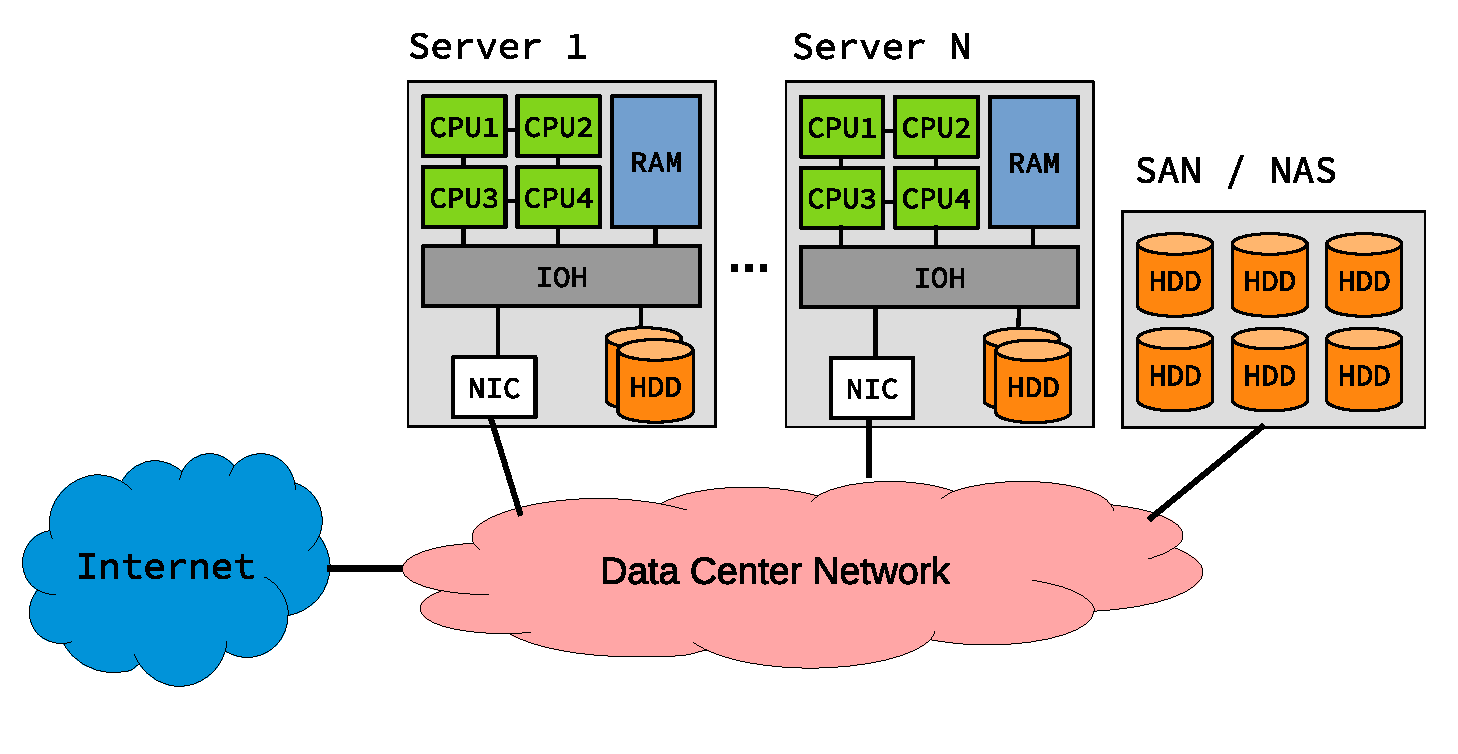
\includegraphics[scale=0.5]{./background/dc_architectures_conventional.eps}

\end{figure}

\end{frame}


\begin{frame}
	Proposed disaggregated data center architecture (\cite{7830659})
\begin{figure}
	\centering
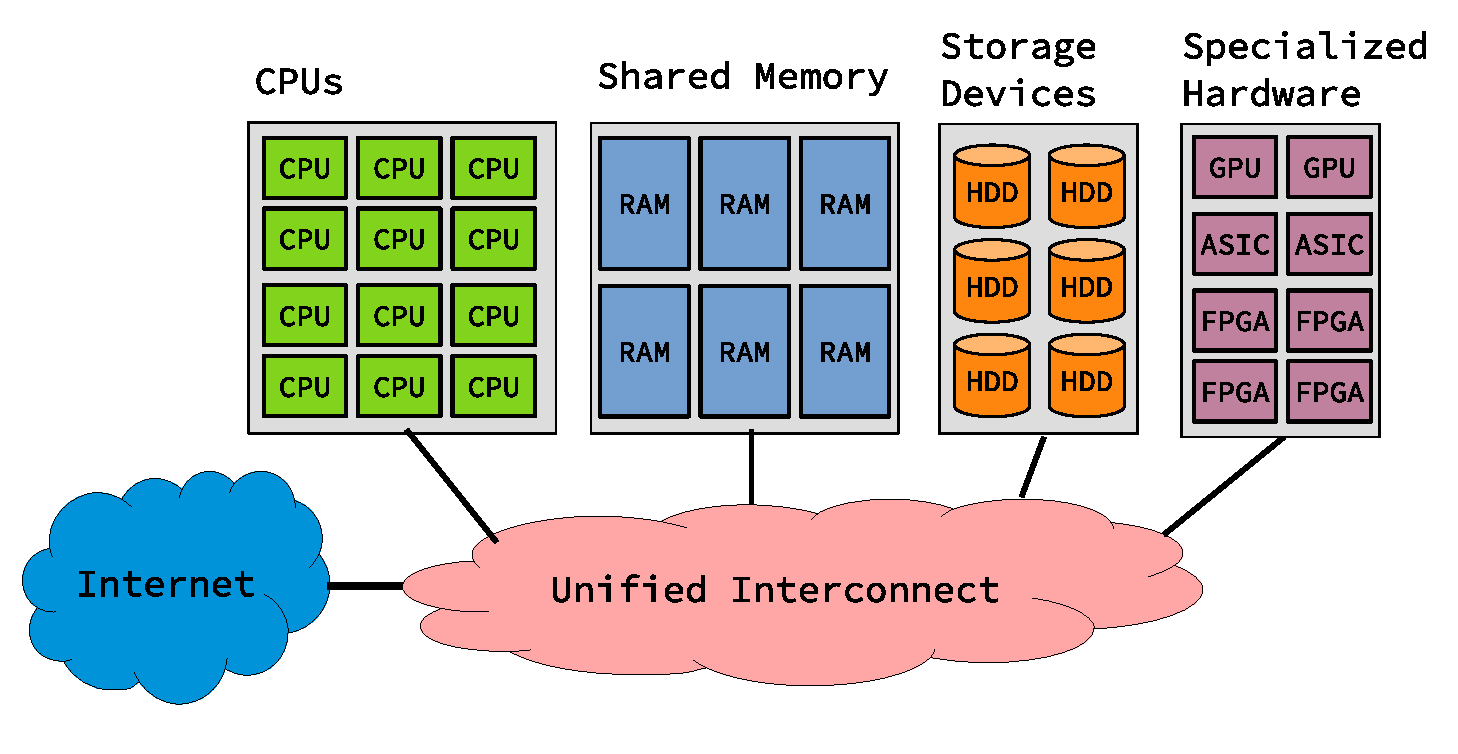
\includegraphics[scale=0.5]{./background/dc_architectures_disaggregated.eps}
\end{figure}
\end{frame}

\note{Hvis man splitter resourcerne op, kan man takket været FPGA få bedre
ydeevne på det samme areal, samt nemmere håndtering af servere og deres komponenter. }

\begin{frame}
FPGA usage
\begin{figure}
	\centering
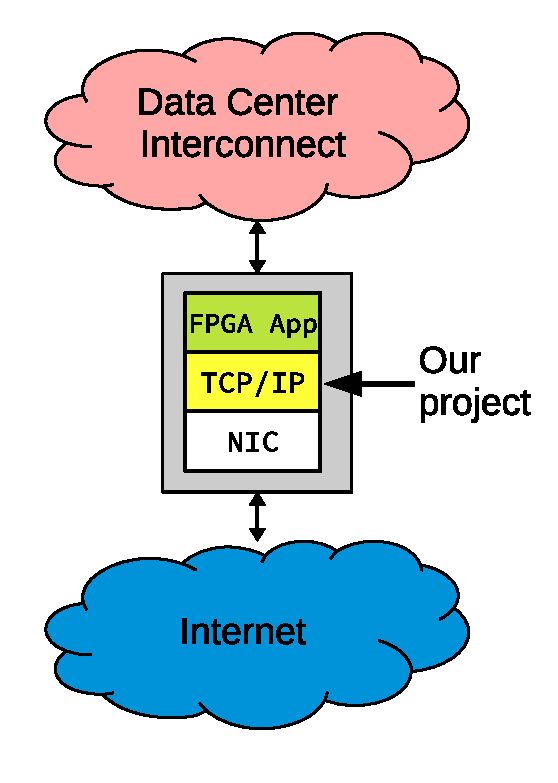
\includegraphics[scale=0.5]{./background/fpga_usage.eps}
\end{figure}

\end{frame}

\begin{frame}
The Internet

\begin{figure}
	\centering
\includegraphics[scale=0.18]{./background/internet_map.jpg}
\label{fig: Internet map}
\caption{Map of the 30\% of accessible the endpoints on the Internet}
\end{figure}

\end{frame}


\begin{frame}
The Internet Protocol Suite -- A scenario
\begin{figure}
	\centering
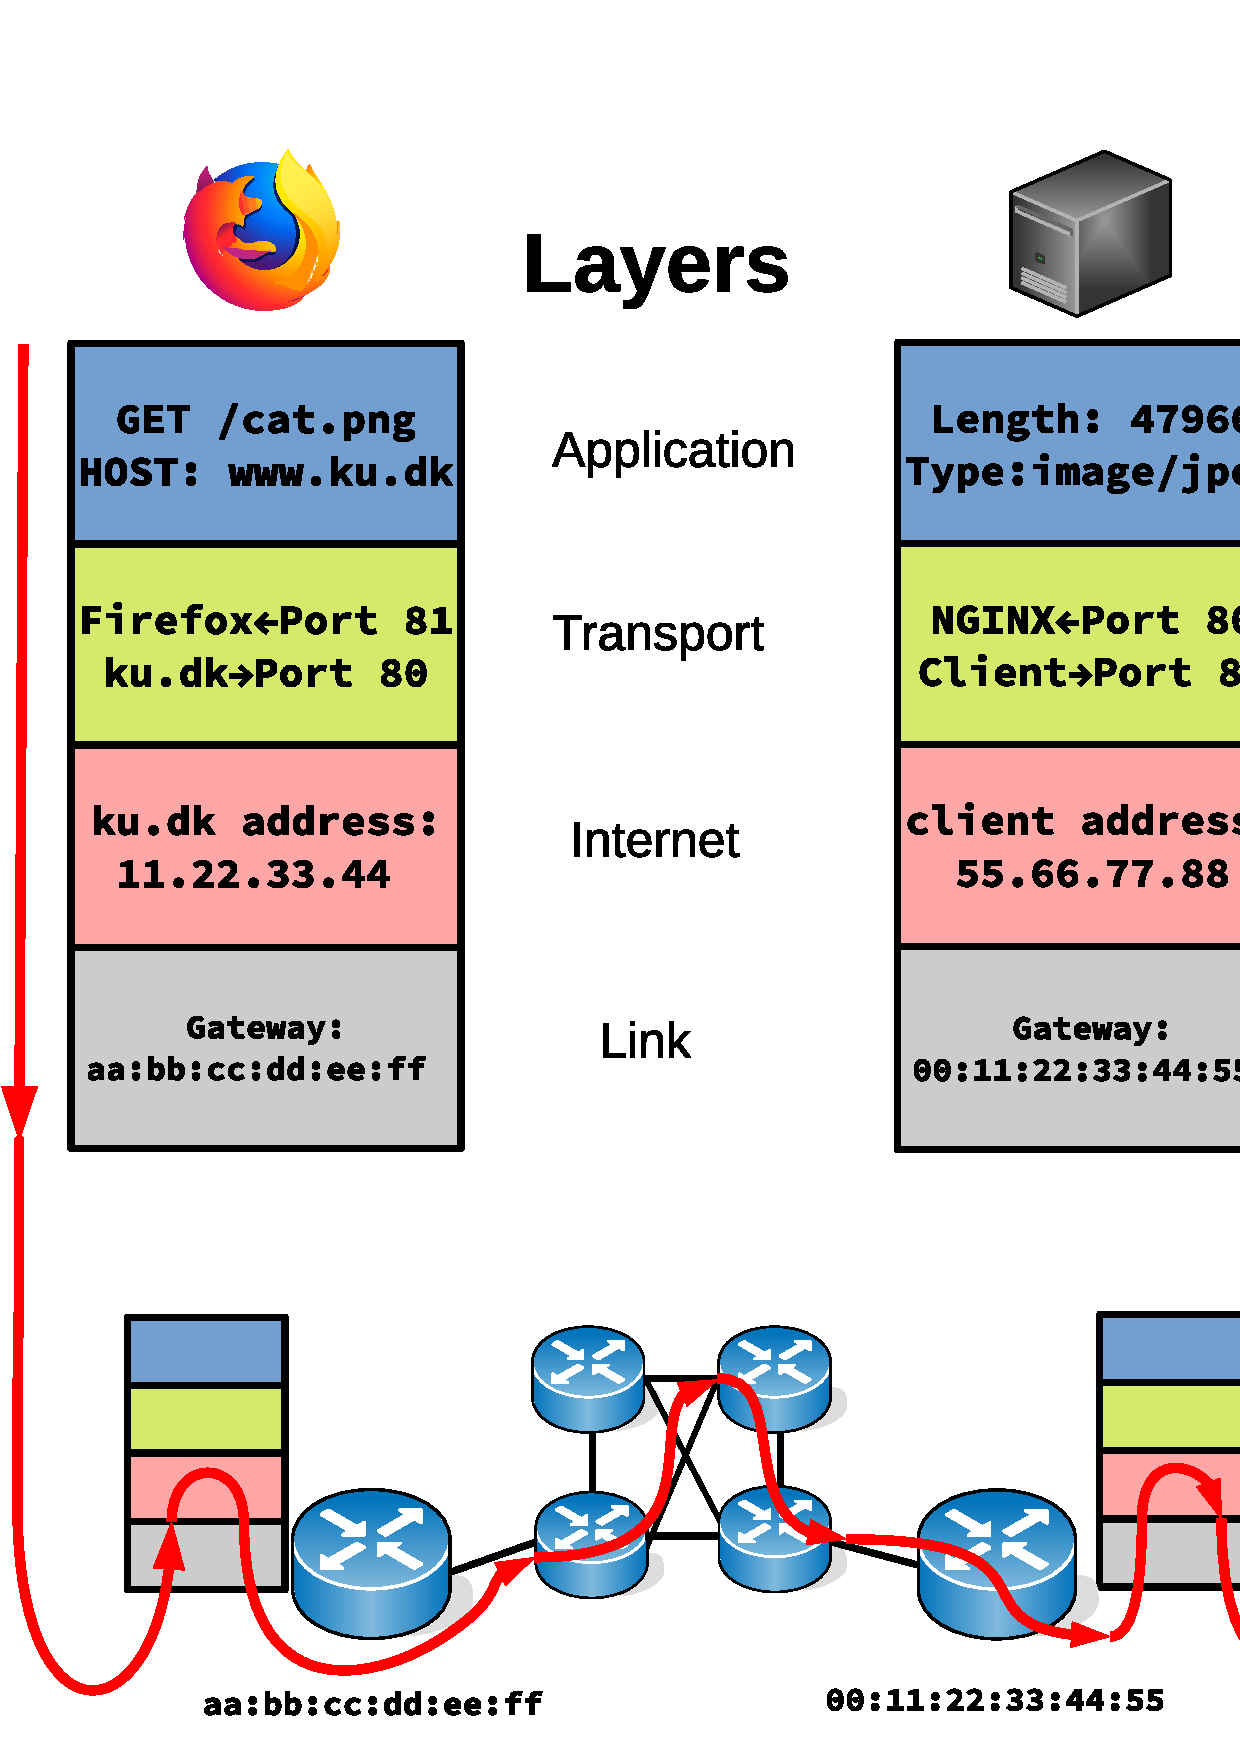
\includegraphics[scale=0.28]{./background/internet_scenario.pdf}
\end{figure}



\end{frame}


\begin{frame}
Design with the 4 layers in mind
\begin{figure}
	\centering
%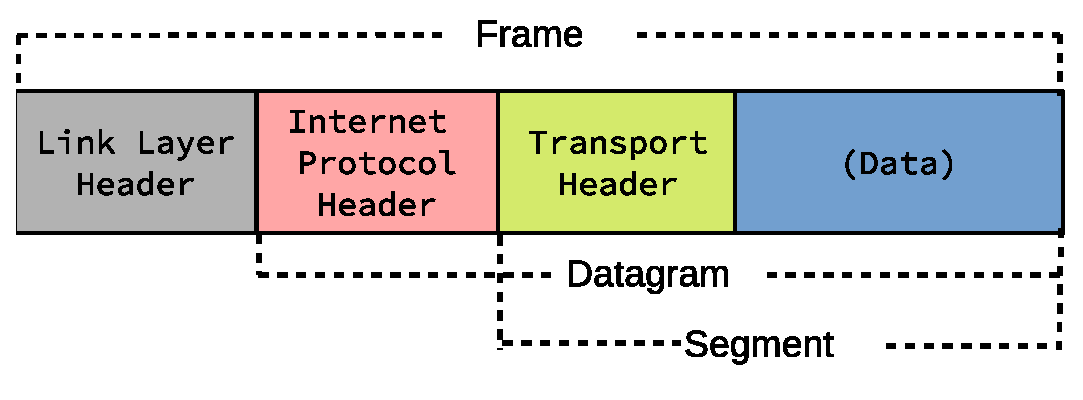
\includegraphics[scale=0.5]{./background/frame.eps}
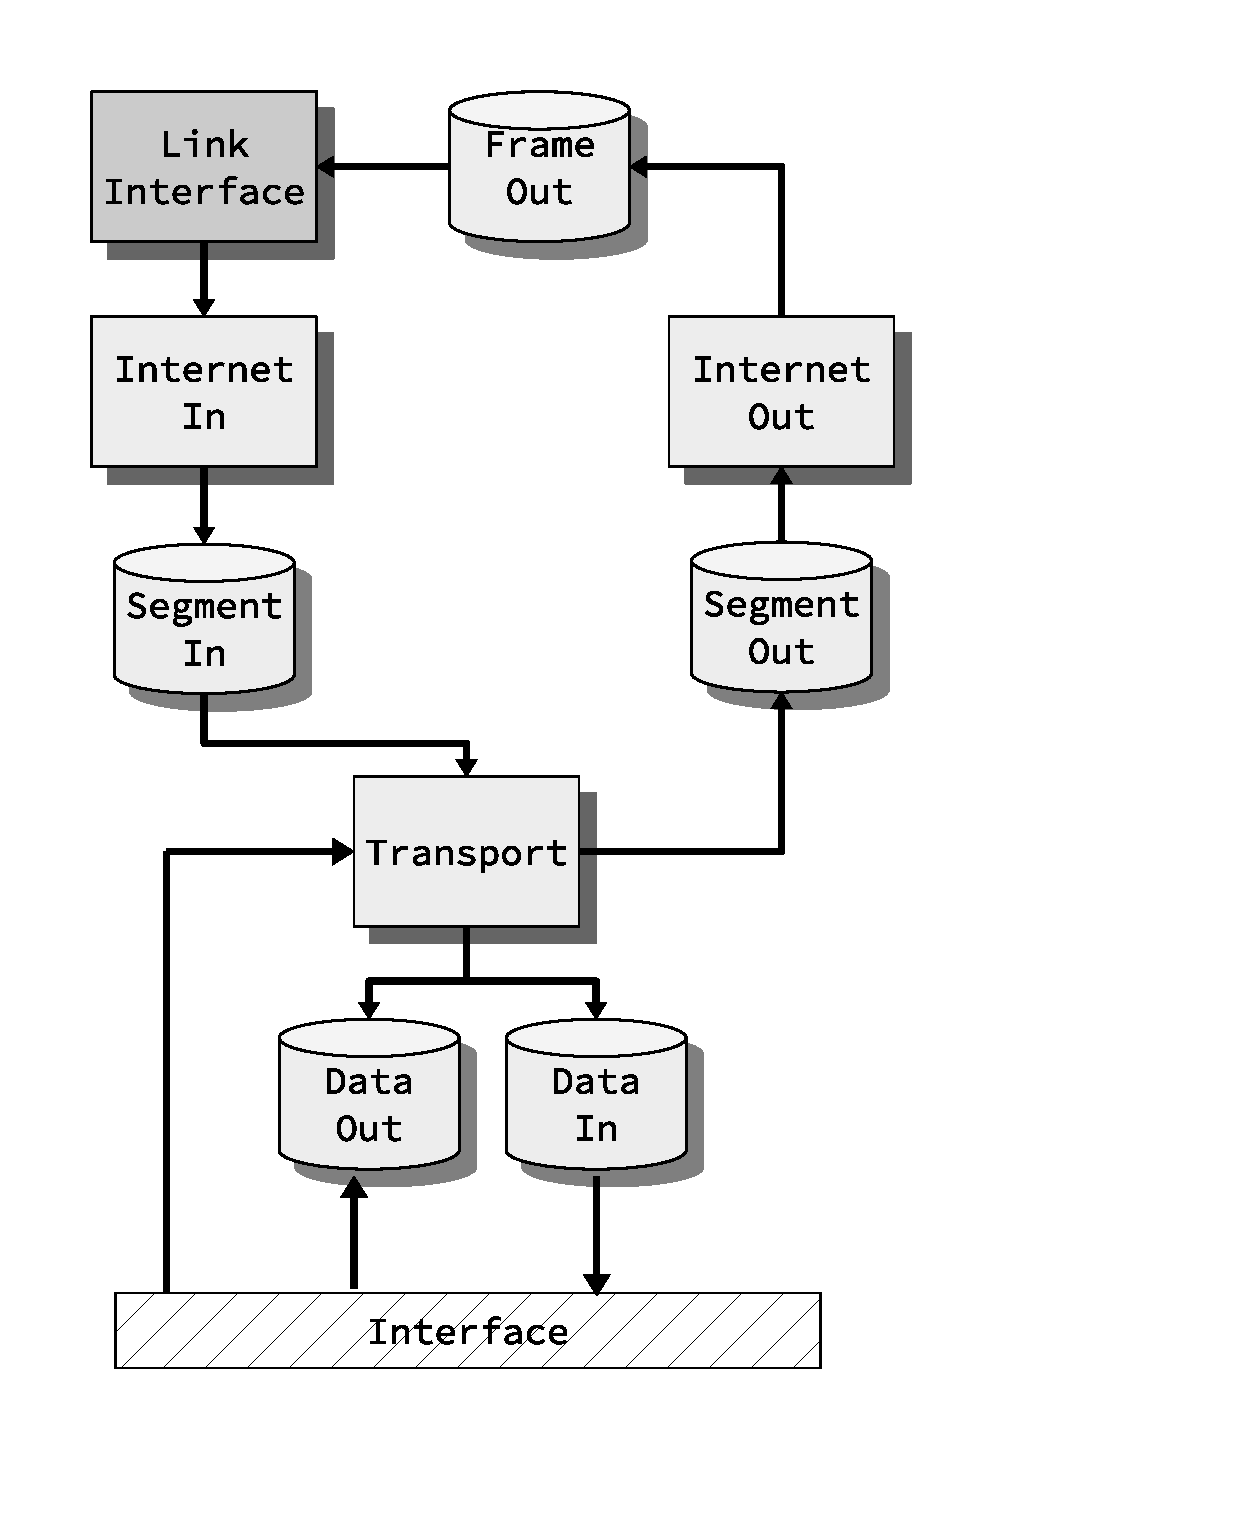
\includegraphics[scale=0.3]{./background/design_2.eps}
\end{figure}
\end{frame}



% - Network Stack Specialization for Performance\\
% - Disaggregated FPGAs\\
% - A Cloud-Scale Acceleration Architecture

% Talking points:
% 1. In the current era of big data, computationally heavy applications are
% moving to the cloud.

% 2. DC infrastructures are being redesigned to pack ever more compute capacity
% into the same volume and power envelops

% 3. This is done by increasing the density of the servers by sharing resources,
% such as power supplies, cooling, fans, networking uplinks, and other management
% infrastructures.

% 4. Problem -- currently, FPGAs are connected directly to CPUs using some PCI
% bus, making the separation hard. [0] proposes FPGA must be turned into a
% self-contained standalone appliance capable of managing itself. Then, it is
% connected to the rest of the Data-Center by a local network.

% 5. In this thesis, we want to make a self-contained TCP/IP stack on an FPGA
% using SME.


% [0]: [Disaggregated FPGAs]



\chapter{Design}
% introduction about the network stack?

\section{Overview}
The networking stack introduced in this thesis is implemented in the C\# 
programming language with SME. The aim of its design is to capacitate performance,
flexibility, and ease of use. In this chapter, the design principles are 
described, the architecture of the solution is outlined, and the components are
outlined.


\subsection{Design principles}
As briefly mentioned in the introduction, the proposed network stack is to 
provide an alternative to the existing proprietary network offloading engines.
While the main goal of this thesis is to research and study the suitability of 
SME for implementing a TCP/IP stack on an FPGA, there are many other aspects of the 
system to be studied.\\
The extensibility of the network stack are to be tested by studying the effects 
of introducing new protocols to the stack. While the network stack should be 
able to be refined with new and custom protocols, it is to be studied which 
implications it has for the system. Mainly, it is to be seen how the addition 
of new protocols affect the performance, scalability, and viability of the 
system.\\
In the same vein, the design should be as FPGA-agnostic as possible. While this is 
mainly guaranteed by the SME framework used to develop the system, the underlying
systems, operations, and features should be easily portable across FPGA manufacturers.\\
Lastly, the design of the networking stack should be interoperable with other 
systems on the FPGA, or even FPGAs. It is to be seen how easy it us to modify
and extend the versatility of the system without any major modifications or 
even extensible knowledge of the system. As an example, the networking stack 
can be expanded with a firewall, developed alongside this project. 

\subsection{Initial requirements}
Following our design principles, initial requirements and goals for the 
networking stack are set so that these can be tested and improved upon. 
\begin{itemize}
\item \textbf{Essential protocols only}\\
Considering that the SME project is still fairly early in its development, and considering 
the sheer number of protocols in the internet protocol suite, the networking 
stack in this thesis is to support only the absolutely essential protocols 
required to provide the users with a meaningful interface to the internet.
These protocols should be picked such that the system can provide the end-user
with a network data-stream, which can transport information to and from a remote
computer.\\
The initial protocols chosen may be implemented and supported partially, but 
they must not deviate from the standard specifications. 

\item \textbf{Support an interface for the end-user}\\
The system must be controlled by an end-user on the FPGA. Such an interface is 
very unique in its own way, compared to standard software interfaces, like the 
ones defined in the POSIX collection of specifications. By supporting such an
external interface gains insight in the way such a networking stack will be used,
and which measures must be taken in order to provide the best possible integration
and performance considerations.

\item \textbf{Independent of underlying physical hardware}\\
By using SME, the underlying hardware description language code can be abstracted
away from the actual implementation. This will later provide developers to easily
modify and tweak the networking stack without having to consider the target 
hardware.\\
Likewise, the networking stack may not rely on using a certain physical layer hardware,
and must be designed to be independent of the underlying hardware used for the 
physical connections. This will ensure that the target hardware can easily 
swap between physical connectors, such as going from ethernet cables to wireless,
or even another FPGA.
\end{itemize}

\section{The architecture}
\subsection{Initi1al design}

\begin{figure}
    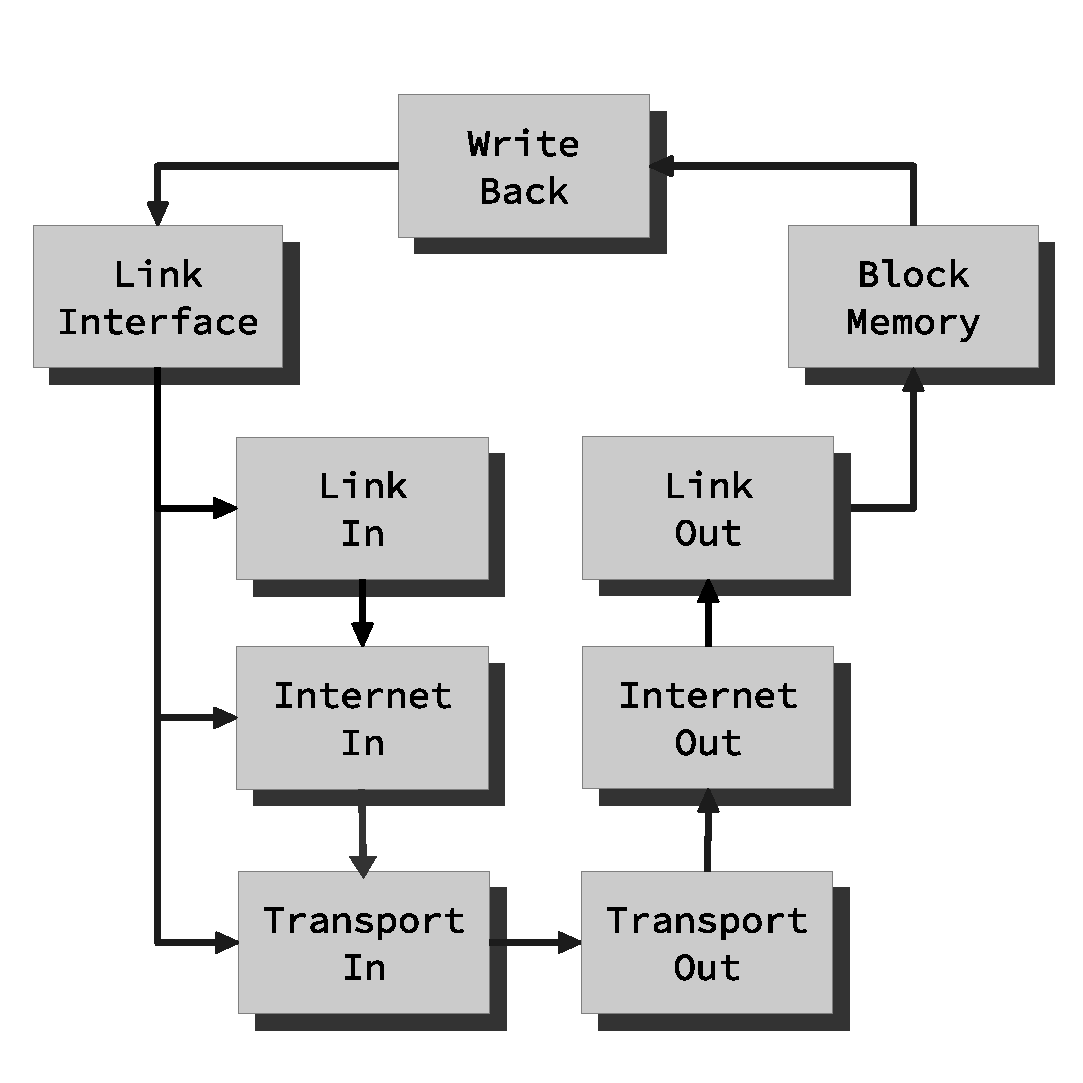
\includegraphics[scale=0.45]{design/design_0.eps}
    \caption{The initial design}
    \label{fig:initial_design}
\end{figure}

The initial architecture focused heavily on the input from the link interface, 
minimizing hardware memory requirements, and to minimize the latency from the 
source data-stream to its respective layer handler.\\
In the initial design, figure \ref{fig:initial_design}, the link interface, which
provides the raw byte-stream from the network, is connected to all of the input
parsing layers. The layers are connected in the order in which a network frame 
is parsed; link- to internet- to transport-layer. This approach aims to utilize
the fact that the layers can act immediatelly upon the packets received directly
from the source, avoid having to buffer the whole packet in each stage, as well 
as easing the logic required to buffer the data across the layers.\\
This design starts by the Link Interface sending one byte at a time through its bus. 
The \texttt{Link In} will parse the first header, and signal the next layer upon completion.
\texttt{Internet In} will then start to listen on the \texttt{Link Interface} bus
and, using the information from \texttt{Link In}, parse the internet header 
accordingly. The same procedure would be applied to the connection between 
\texttt{Internet In} and \texttt{Transport In}.\\
When data is to be sent to the internet, the network frame would be built bottom
up from the transport layer through internet to the link layer.

\subsubsection{The issues}
The issues quickly surfaced during the implementation of the design. Although 
the interconnect from the \texttt{Link Interface} to all the subsequent layers
in parallel promised negligible latency, it came with a great cost to the solution:
\begin{enumerate}

\item \textbf{Process under-utilization} \label{item:process_utilization}\\
Since each "in" process has to wait for the previous layer to signal when to 
start listening on the data-bus, the layers would in average only be active a third
of the time. Since each layer has very little information about the states of 
the other layers, it would become a challenge to get any other work done during
these phases.\\
For example, it would be an immense challenge to coordinate an ICMP reply on a 
faulty packet in the \texttt{Internet In}.

\item \textbf{Redundant Link layer}\\
While the Link layer is an essential part of the Internet Protocol Suite, it did 
not fit well with the functionality of the rest of the stack. 
Most network interfaces are equipped with buffers, on which integrated circuits
perform operations such as error check using cyclic redundancy check, de-noising,
timeslot management, etc. 
Likewise, the Pmod NIC100 Ethernet interface has built-in controller with 
internal memory suited for buffering the incoming packets\cite{microchip_enc424j600}.
This memory, apart from the cyclic redundancy check, can be used as the initial
step for parsing the packet, and only send the datagram to the stack.


\item \textbf{IPv4 fragmentation and out of order TCP packets}\\
The chaotic nature of internet routing might cause packets to come out of order,
or even get fragmented along the way. Since each layer parses the packet immediatelly
as it is written to the bus, it became a challenge for the layers to figure out 
what to do. On IPv4 fragmentation, if the second half of a dataframe arrived 
first, the Transport header would not be available to the Transport layer. 
Although IPv4 fragmentation is an increasingly rare phenomenon, the network 
design is not able to handle the situation well.  

\cofeAm{0.7}{0.75}{2}{80}{0}


\item \textbf{TCP connection state sharing}\\
With a clear separation between the "in" layers and the "out" layers, the 
Transport block had to be split as well. Unfortunately, unlike the other stateless
layers, the transportl layer actually needs to keep track of the connections and 
their states. On every segment received, the appropriate connection needs to be 
updated accordingly.\\
In the TCP protocol, the connection state changes on both receiving and sending.
In this case, the \texttt{Transport In} and \texttt{Transport Out} have to 
agree on a shared state. As these states can be quite large, and the should 
support multiple connections at once, one large bus containing all the information
is not feasible. To solve this, a negotiation protocol may be introduced, however,
as pointed out in item \ref{item:process_utilization}, the processes are very
limited in their execution time. A negotiation would be very hard to achieve in 
such circumstances.
% \item \textbf{Control and logic flow} \\
% Although the layers take turns to parse the incoming byte-stream, the design 
% handles the whole packets at once.  

\end{enumerate}

While it would be possible to work around these identified issues in code, the 
added complexity would have additional ramifications on the project as a whole.
Upon further analysis of analysis, it is clear that the source of the issues is 
the parallel arrangement of the process blocks.

\section{Pipelined design}
\begin{figure}
    \includegraphics[scale=0.45]{design/design_1.eps}
    \caption{The revised design}
    \label{fig:revised_design}
\end{figure}

The next iteration of the design utilizes a fairly standard approach to 
pipelining, albeit with an unusual transfer of data between the stages.\\
The idea with the pipeline is to enable the processes to receive, compute, and 
forward data at their own pace, without any major limitation from the other 
parts of the system.


\subsection{Internet layer processes} \label{sec:layer_processes}
The processes performing computation and processing on the actual internet 
packets, called "layer processes" for brevity, are by large kept intact from the 
previous design. The fairly simple, but highly sequential nature of packet 
header parsing turned out to be very complicated to optimise with the additional
computing power of the hardware, without introducing too much complication.\\
Missing from the updated figure \ref{fig:revised_design} are the \texttt{Link In}
and \texttt{Link Out} processes, which, for now, are made by the ethernet 
interface, which can easily parse and strip the first frame headers.


\subsection{Data buffers} \label{sec:data_buffers}
Illustrated as cylinders on figure \ref{fig:revised_design}, First-In, First-Out (FIFO)
buffers are introduced between each parsing process in order to control the data-flow 
between the layers. Apart from maintaining a fairly large memory bank through 
the block-RAM, these buffers also contain logic to store the incoming data
intelligently in order to offload the following processes. For example, the
\texttt{Segment In} buffer ensures that fragmented IPv4 packets are defragmented
before leaving the buffer.
However, introducing a new "type" of a process --- the buffers --- poses a new 
challenge. While the buffers can be read from at any time, the layer-parsing
processes do not have this luxury, as they do not have any significant internal
buffer. Hence, a consistent handshake and data-exchange interface signal protocols
are needed.

\subsection{Interface Signal protocols}
With the introduction of buffers between each parsing processes, a clear pattern
emerged. The layer-handling processes are responsible for numerous real-time tasks 
(parsing, sending, protocol-specific tasks, etc), while also limited by their 
fixed internal buffers. These processes are not always ready to receive input 
from preceding processes, while they at the same time must be able to write their
output to following processes immediatelly.\\
The buffers are a stark opposite, as their large internal block memories enable
them to buffer huge chunks of memory, while also being able to wait for the 
succeeding process to start reading.\\
With these two established scenarios, protocols for each can be proposed.  

\subsection{Buffer-Producer data transfer}

\subsection{Compute-Producer data transfer}

% \cofeAm{0.7}{0.75}{2}{80}{0}


\section{Implementation}
\newcommand{\ImplementationTitle}{Implementation}
% \begin{frame}
%     \frametitle{\ImplementationTitle}
%     \centering
%     \begin{minipage}{1\textwidth}
%         \begin{itemize}%[<+->]
%             \item SME introduction
%             \item Processes
%             \begin{itemize}
%                 \item State machines
%             \end{itemize}
%             \item Buffers
%             \begin{itemize}
%                 \item Memory segments
%                 \item Dictionary
%             \end{itemize}
%             \item Interface signal control
%             \begin{itemize}
%                 \item Buffer-Producer
%                 \item Compute-Producer
%             \end{itemize}
%         \end{itemize}
%     \end{minipage}
% \end{frame}

\begin{frame}
    \begin{textblock*}{\displayThumbnail}(\paperwidth-\displayThumbnail-0.2cm,0cm) % {block width} (coords)
        \colorbox{white}{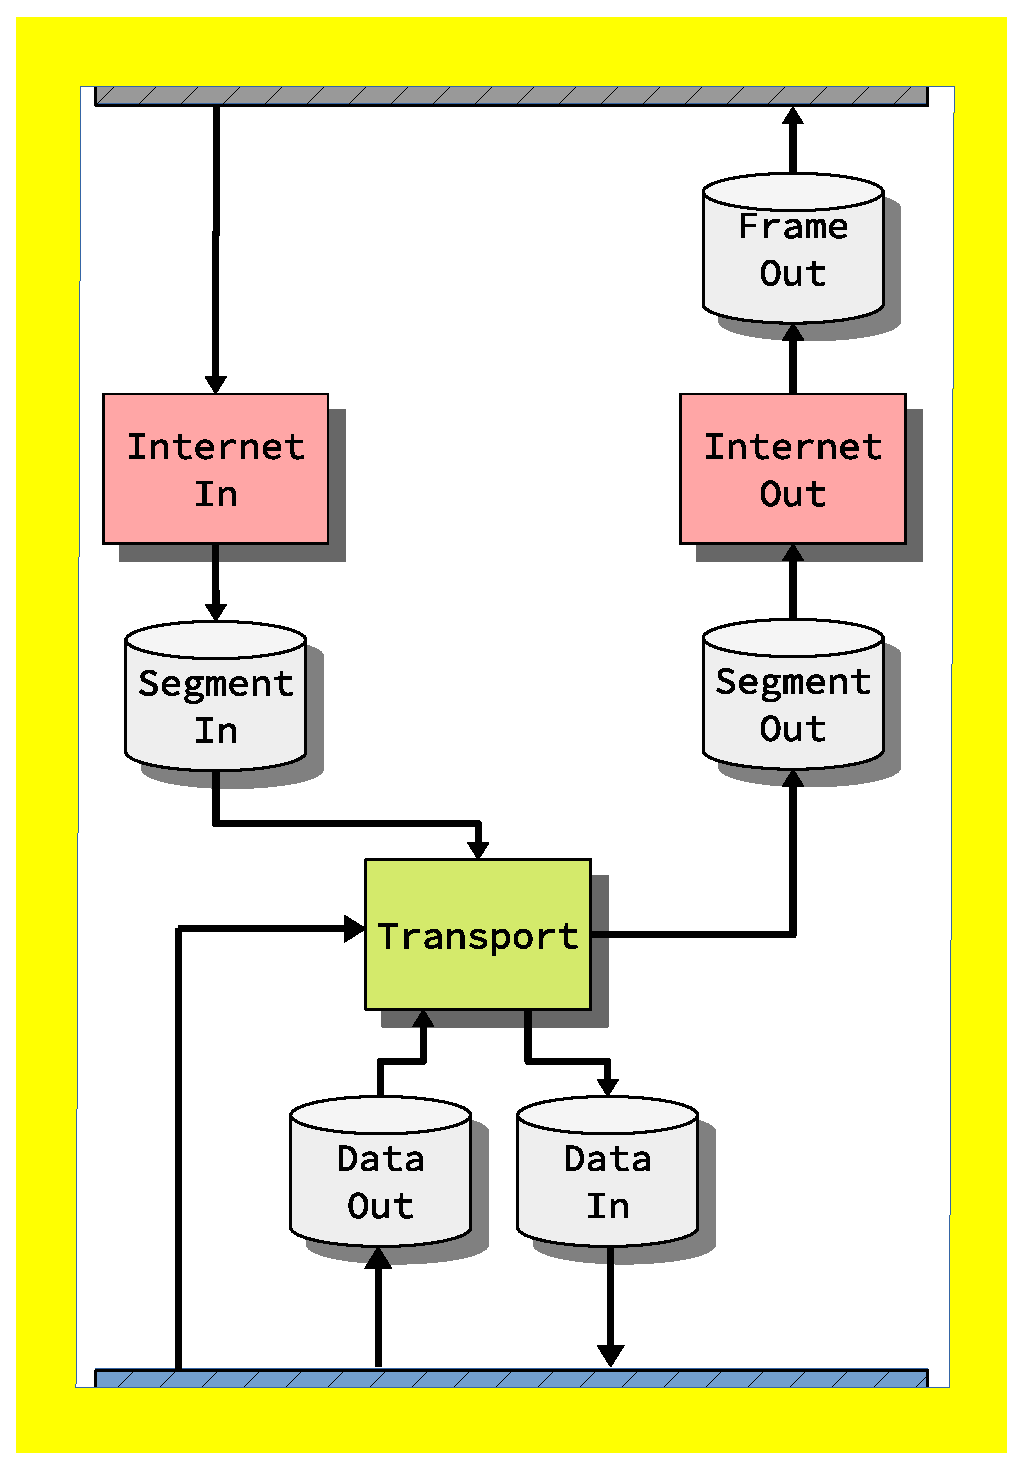
\includegraphics[width=\textwidth]{implementation/design_2_sme.eps}}
    \end{textblock*}
    \frametitle{\ImplementationTitle}
    \subsection{SME introduction}
    \framesubtitle{SME introduction}

    \begin{block}{SME(Synchronous Message Exchange) introduction}
        \begin{itemize}
            \item Processes and Busses
            \item Higher abstraction
            \item Handling of clocks
            \item Easy testing
            \item Not fully feature complete with C\#(No threads, no allocation)
        \end{itemize}
    \end{block}

\end{frame}
\note{
    \begin{itemize}
        \item What is a bus and a process
        \item No VHDL code
        \item Clocks abstracted away behind the management of processes and busses
        \item Testing straight in the simulator, but also in afterwards in the GHDL
              compiler, via an clock lookup table
        \item Since not feature complete, only simple structures can be used. We choose
              state diagrams since they are possible to make, and easy to understand
    \end{itemize}
}
\begin{frame}[fragile]
    \begin{textblock*}{\displayThumbnail}(\paperwidth-\displayThumbnail-0.2cm,0cm) % {block width} (coords)
        \colorbox{white}{\includegraphics[width=\textwidth]{implementation/design_2_state.eps}}
    \end{textblock*}
    \frametitle{\ImplementationTitle}
    \subsection{Processes}
    \framesubtitle{Processes}
    State machines\\\\
    %\begin{onlyenv}<2>
    \begin{minipage}[t]{0.3\textwidth}
        \begin{mintedcsharp}
            public class SomeProcess : StateProcess
            {
              private override async Task OnTickAsync()
              {
                a();
                await ClockAsync();
                b();
                await ClockAsync();
                c();
                await ClockAsync();
              }
            }
        \end{mintedcsharp}
    \end{minipage}%
    %\end{onlyenv}%
    \hfill%
    \begin{minipage}[t]{0.3\textwidth}
        \begin{mintedcsharp}
            public class SomeProcess : SimpleProcess
            {
            // Initial state
            state = A;

            protected override void OnTick()
            {
              switch(state) {
                case A:
                  a();
                  state = B;
                case B:
                  b();
                  state = C;
                case C:
                  c();
                  state = A;
              }
            }
        \end{mintedcsharp}
    \end{minipage}%
    \hfill%
    \begin{minipage}[t]{0.3\textwidth}
        \begin{figure}
                \centering
                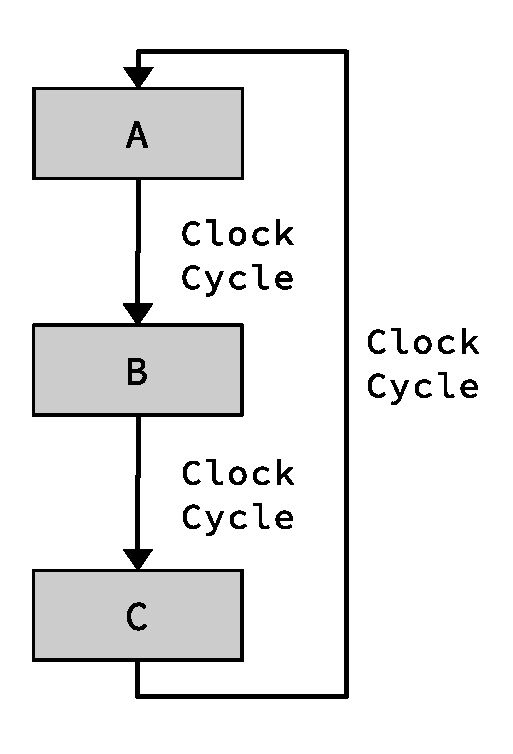
\includegraphics[scale=0.45]{implementation/empty_process_fsm.eps}
        \end{figure}
    \end{minipage}
    %\Put(-50,0){\colorbox{white}{\includegraphics[width=0.2\textwidth]{implementation/design_2_state.eps}}}

\end{frame}

\note{
State machines\\
\begin{itemize}
    \item \texttt{StateProcess}\\
          Eksekvering kan stoppes når som helst(i bidder)
    \item \texttt{SimpleProcess}\\
          Run er en clock altid, state machine håndteres
          med en switchcase. Algoritme kan splittes op i flere bidder,
          men kræver en state per bid

\end{itemize}
}

\begin{frame}[fragile]
    \begin{textblock*}{\displayThumbnail}(\paperwidth-\displayThumbnail-0.2cm,0cm) % {block width} (coords)
        \colorbox{white}{\includegraphics[width=\textwidth]{implementation/design_2_state_specific.eps}}
    \end{textblock*}
    \frametitle{\ImplementationTitle}
    \framesubtitle{Processes}
    Examples\\
    \begin{minipage}[t]{0.5\textwidth}
        \begin{figure}
            \centering
            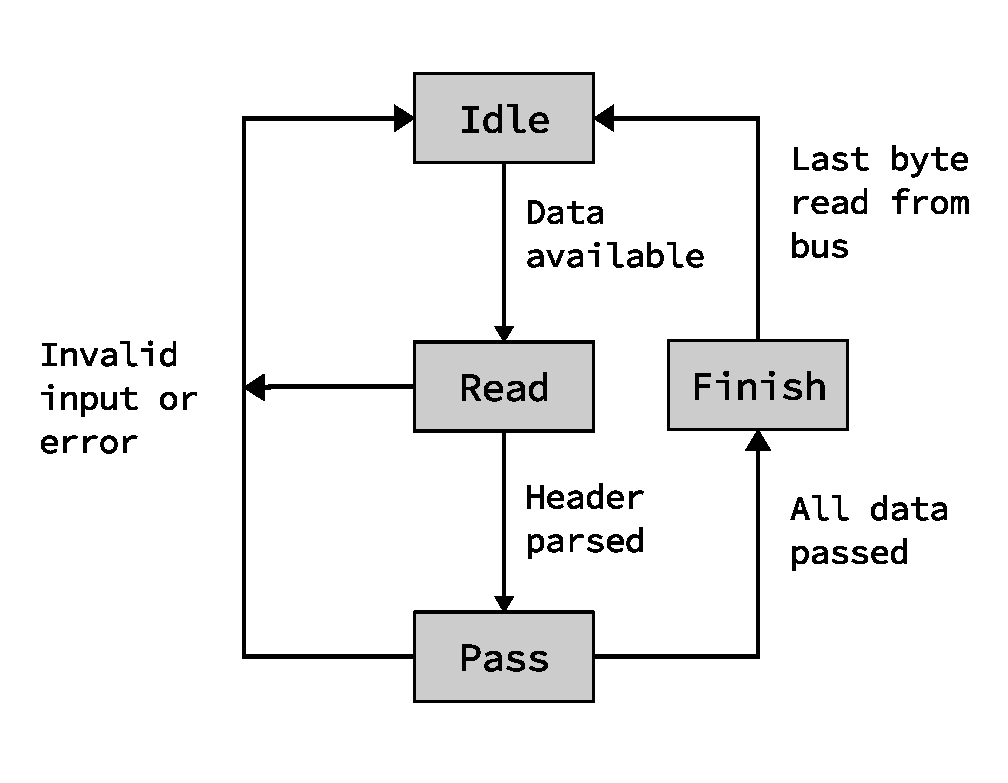
\includegraphics[scale=0.35]{implementation/internet_in_fsm.eps}
            Internet in process state machine
        \end{figure}
    \end{minipage}%
    \hfill%
    \begin{minipage}[t]{0.5\textwidth}
        \begin{figure}
            \centering
            \includegraphics[scale=0.35]{implementation/transport_fsm.eps}
            Transport process state machine
        \end{figure}
    \end{minipage}
\end{frame}
\note{

    \begin{itemize}
        \item Gå igennem state diagrammer
        \item Snak om grundlaget for de forskellige typer brug
    \end{itemize}
}

\begin{frame}[fragile]
    \begin{textblock*}{\displayThumbnail}(\paperwidth-\displayThumbnail-0.2cm,0cm) % {block width} (coords)
        \colorbox{white}{\includegraphics[width=\textwidth]{implementation/design_2_memory.eps}}
    \end{textblock*}
    \frametitle{\ImplementationTitle}
    \subsection{Buffers}
    \framesubtitle{Buffers}
    \begin{block}{Why buffers?}
        \begin{itemize}
            \item Fixes segmentation
            \item Processes can get data at their leisure
        \end{itemize}
    \end{block}

\end{frame}
\note{Hvorfor bruer vi buffers?}


\begin{frame}[fragile]
    \begin{textblock*}{\displayThumbnail}(\paperwidth-\displayThumbnail-0.2cm,0cm) % {block width} (coords)
        \colorbox{white}{\includegraphics[width=\textwidth]{implementation/design_2_memory.eps}}
    \end{textblock*}
    \frametitle{\ImplementationTitle}
    \framesubtitle{Buffers}
    Memory segments\\
    \begin{minipage}[t]{1\textwidth}
        \begin{figure}
                \centering
                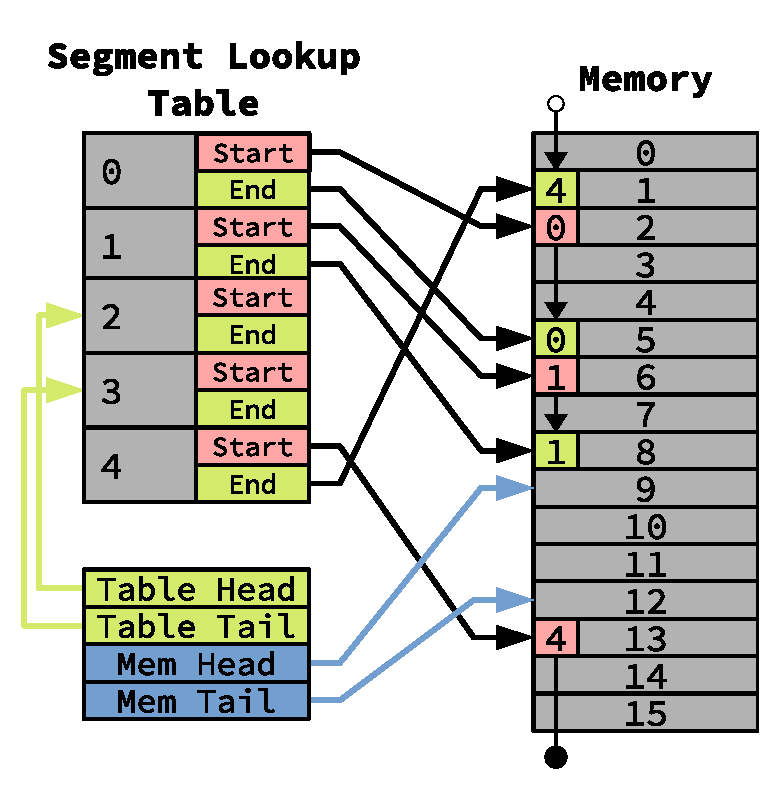
\includegraphics[scale=0.50]{implementation/memory_segments.eps}
        \end{figure}
    \end{minipage}
\end{frame}
\note{
    \begin{itemize}
        \item Reason behind?
        \begin{itemize}
            \item Segment handling
            \item References to other segment to concatting of segments later
        \end{itemize}
    \end{itemize}

}

\begin{frame}[t]
    \note<1->{Snak om input
}
    \begin{textblock*}{\displayThumbnail}(\paperwidth-\displayThumbnail-0.2cm,0cm) % {block width} (coords)
        \colorbox{white}{\includegraphics[width=\textwidth]{implementation/design_2_memory_dictionary.eps}}
    \end{textblock*}
    \frametitle{\ImplementationTitle}
    \framesubtitle{Buffers}
    Memory dictionary
    \begin{columns}[t]
        \begin{column}{0.5\linewidth}
            \begin{figure}
                \centering
                \begin{overlayarea}{\textwidth}{\textheight}
                    \only<1>{\includegraphics[width=\textwidth]{./implementation/memory_dictionary/memory_dictionary_multi_0.eps}}
                    \only<2>{\includegraphics[width=\textwidth]{./implementation/memory_dictionary/memory_dictionary_multi_1.eps}}%
                    \only<3>{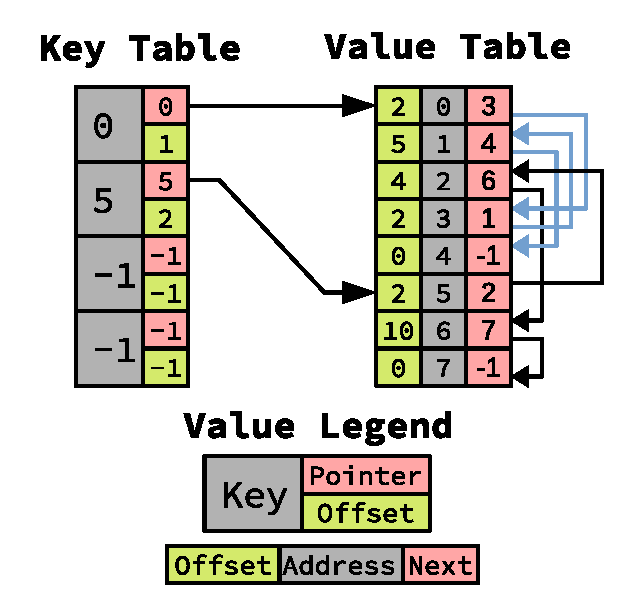
\includegraphics[width=\textwidth]{./implementation/memory_dictionary/memory_dictionary_multi_2.eps}}%
                \end{overlayarea}
            \end{figure}
        \end{column}

        \begin{column}{0.3\linewidth}
            \\
            \only<1>{
                Initial state.\\
                Key \texttt{5} have 2 elements:\\
                $$[4,18]$$
                at index:
                $$[2,7]$$
            }
            \only<2>{
                Insert element 8:
                Key \texttt{5} have 3 elements:\\
                $$[4,8,18]$$
                at index:
                $$[2,6,7]$$
            }
            \only<3>{
                Insert element 2:
                Key \texttt{5} have 4 elements:\\
                $$[2,4,8,18]$$
                at index:
                $$[5,2,6,7]$$
            }
        \end{column}
        \begin{column}{0.2\linewidth}
        \end{column}
    \end{columns}
\end{frame}



\begin{frame}[fragile]
    \note<1->{Overflow!\\
    kan læses ved:
    \begin{itemize}
        \item Kør løkken en gang per clock
        \item Brug en anden model end en linked list, måske et fast offset?
    \end{itemize}
    }
    \begin{textblock*}{\displayThumbnail}(\paperwidth-\displayThumbnail-0.2cm,0cm) % {block width} (coords)
        \colorbox{white}{\includegraphics[width=\textwidth]{implementation/design_2_memory.eps}}
    \end{textblock*}
    \frametitle{\ImplementationTitle}
    \framesubtitle{Buffers}
    Some problems with the memory dictionaries!
    \begin{figure}
        \centering
        \begin{overlayarea}{0.76\textwidth}{\textheight}
            \only<1>{\includegraphics[width=\textwidth]{./implementation/memory_overrun/memory_overrun_0.eps}}
            \only<2>{\includegraphics[width=\textwidth]{./implementation/memory_overrun/memory_overrun_1.eps}}%
            \only<3>{\includegraphics[width=\textwidth]{./implementation/memory_overrun/memory_overrun_2.eps}}%
            \only<4>{\includegraphics[width=\textwidth]{./implementation/memory_overrun/memory_overrun_3.eps}}%
            \only<5>{\includegraphics[width=\textwidth]{./implementation/memory_overrun/memory_overrun_4.eps}}%
            \only<6>{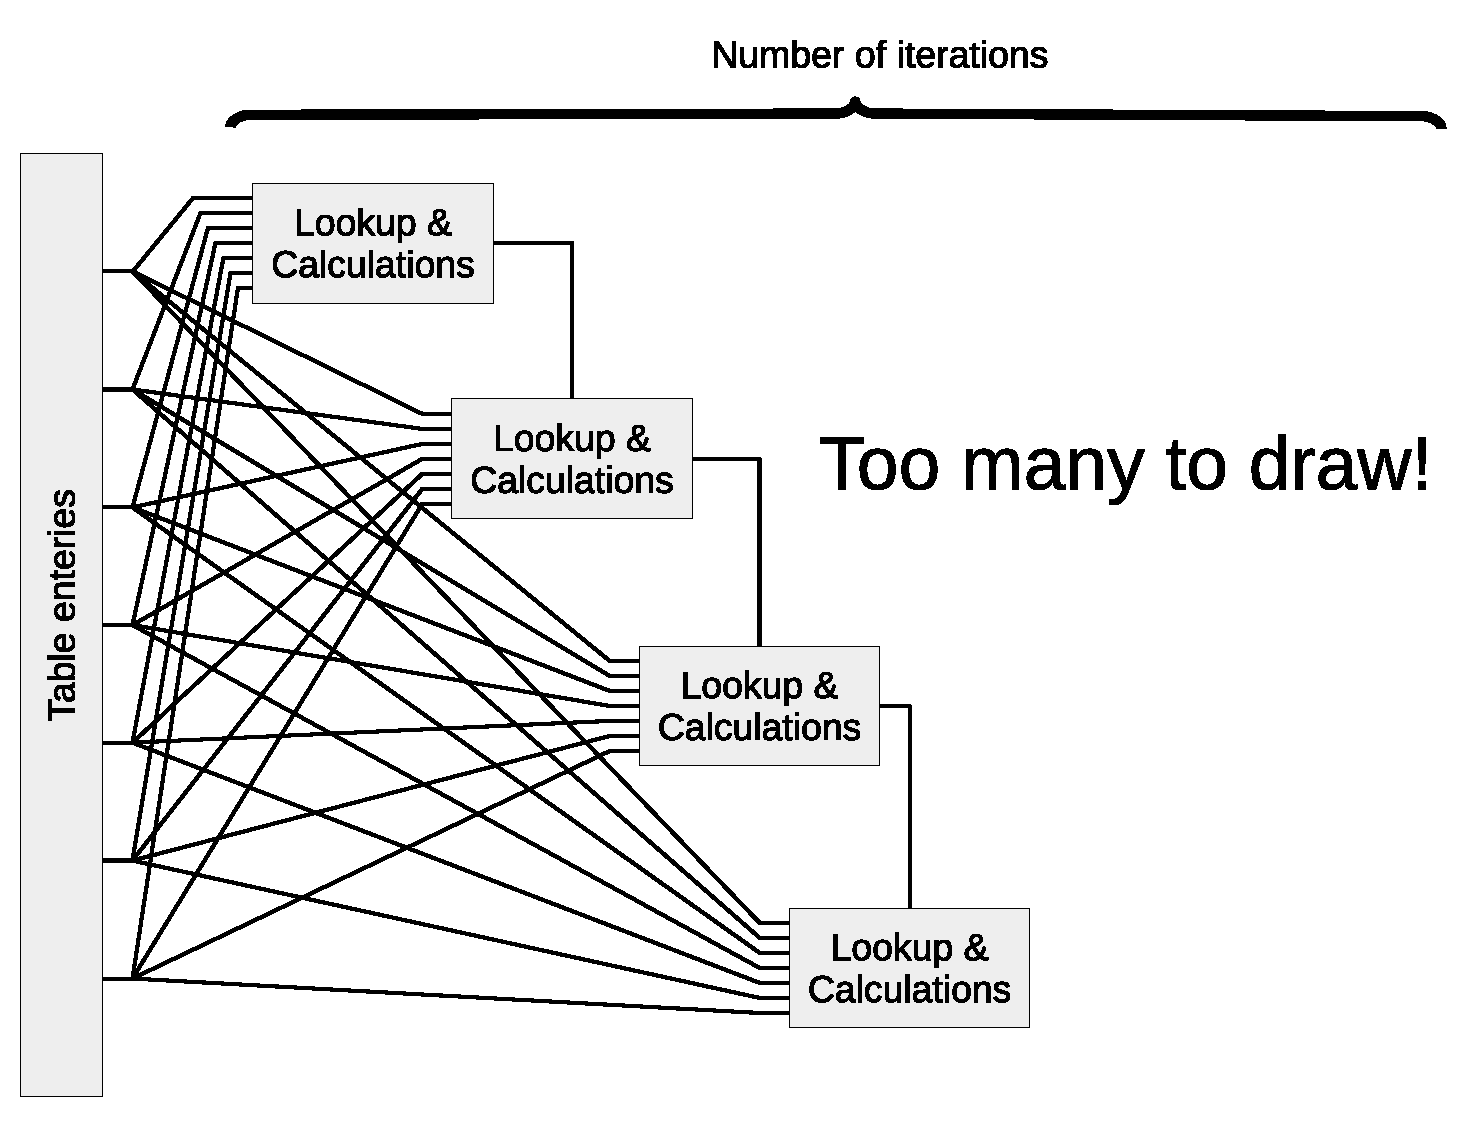
\includegraphics[width=\textwidth]{./implementation/memory_overrun/memory_overrun_5.eps}}%
        \end{overlayarea}
    \end{figure}
\end{frame}


\begin{frame}[fragile]
    \begin{textblock*}{\displayThumbnail}(\paperwidth-\displayThumbnail-0.2cm,0cm) % {block width} (coords)
        \colorbox{white}{\includegraphics[width=\textwidth]{implementation/design_2_busses.eps}}
    \end{textblock*}
    \frametitle{\ImplementationTitle}
    \subsection{Interface signal protocol}
    \framesubtitle{Interface signal protocol}
Identifying the scenarios

\centering
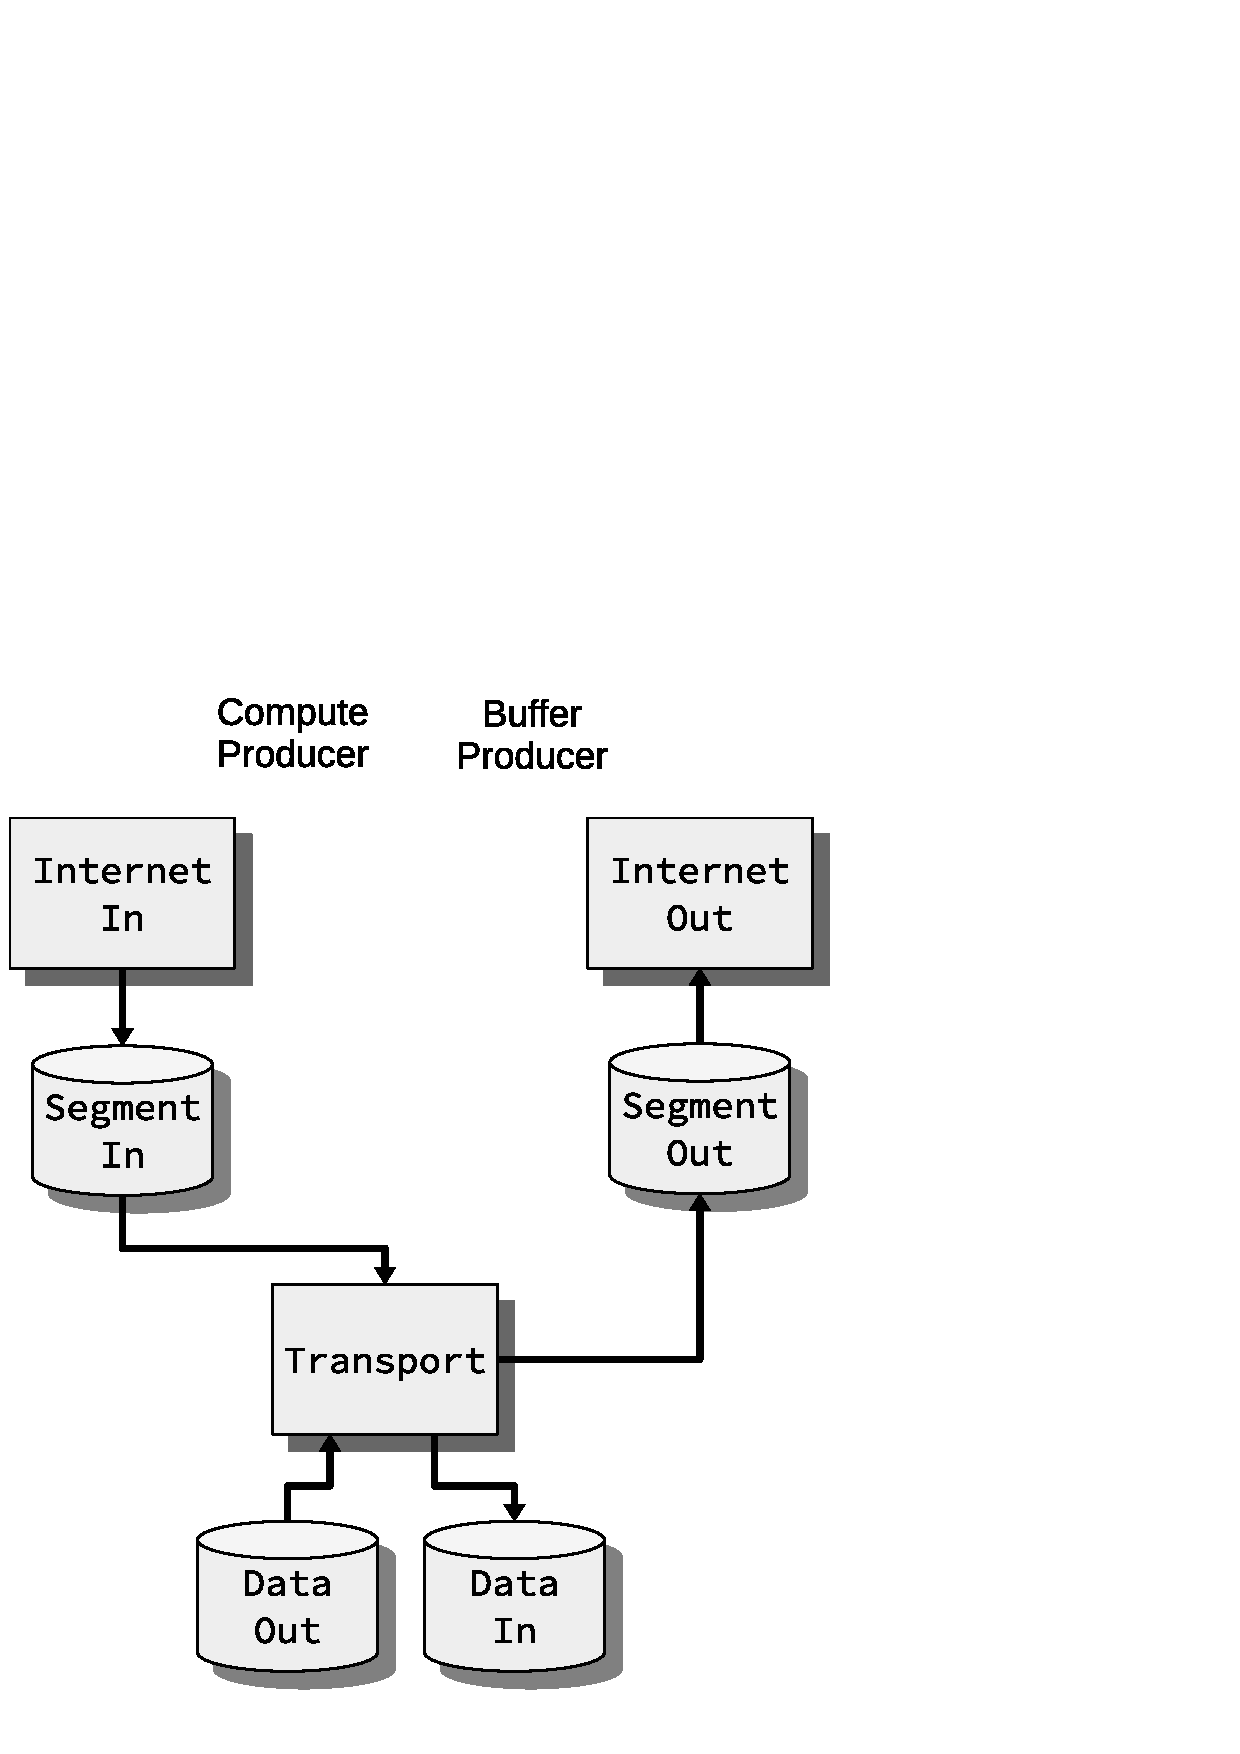
\includegraphics[scale=0.40]{implementation/signal_protocol_identification.pdf}

\end{frame}

\note{Data skal overføres hurtigst muligt, og det må ikke gå tabt\\

2 scenarier: fra "compute" til buffer, og omvendt \\

- CP kan ikke vente\\
- BP har stor buffer, og consumer starter transaktion


}


\begin{frame}[fragile]
    \begin{textblock*}{\displayThumbnail}(\paperwidth-\displayThumbnail-0.2cm,0cm) % {block width} (coords)
        \colorbox{white}{\includegraphics[width=\textwidth]{implementation/design_2_busses.eps}}
    \end{textblock*}
\frametitle{\ImplementationTitle}
\framesubtitle{Interface signal protocol}
\begin{figure}
        \centering
        \includegraphics[scale=0.35]{implementation/compute_producer.eps}
\end{figure}

\end{frame}




\begin{frame}[fragile]
    \begin{textblock*}{\displayThumbnail}(\paperwidth-\displayThumbnail-0.2cm,0cm) % {block width} (coords)
        \colorbox{white}{\includegraphics[width=\textwidth]{implementation/design_2_busses.eps}}
    \end{textblock*}
    \frametitle{\ImplementationTitle}
    \framesubtitle{Interface signal protocol}
    \textbf{Buffer-Producer:} Inspired by AXI4\\
    \begin{figure}
                \includegraphics[scale=0.7]{implementation/axi4_handshake.eps}

        \end{figure}
\end{frame}


\begin{frame}[fragile]
    \begin{textblock*}{\displayThumbnail}(\paperwidth-\displayThumbnail-0.2cm,0cm) % {block width} (coords)
        \colorbox{white}{\includegraphics[width=\textwidth]{implementation/design_2_busses.eps}}
    \end{textblock*}
    \frametitle{\ImplementationTitle}
    \framesubtitle{Interface signal protocol}
        \begin{figure}
                \centering
                \includegraphics[scale=0.35]{implementation/buffer_producer.eps}
       \end{figure}
\end{frame}




% \begin{frame}[fragile]
%     \frametitle{\ImplementationTitle}
%     \framesubtitle{Interface protocol}
%     The interface structures\\
%     \begin{minipage}[t]{0.4\textwidth}
%         \begin{mintedcsharp}
%             enum InterfaceFunction : byte
%             {
%                 INVALID = 0,
%                 // BIND = 1,
%                 LISTEN = 2,
%                 CONNECT = 3,
%                 ACCEPT = 4,
%                 CLOSE = 7,
%                 // ...
%                 OPEN = 255,
%             }
%
%             struct InterfaceData
%             {
%                 public int socket;
%                 public uint ip;
%                 public byte protocol;
%                 public ushort port;
%             }
%         \end{mintedcsharp}
%     \end{minipage}%
%     \hfill%
%     \begin{minipage}[t]{0.4\textwidth}
%         \begin{mintedcsharp}
%             interface InterfaceBus : IBus
%             {
%                 bool valid;
%                 byte interface_function;
%                 InterfaceData request;
%             }
%
%             interface InterfaceControlBus : IBus
%             {
%                 bool valid;
%
%                 byte exit_status;
%                 byte interface_function;
%                 InterfaceData request;
%                 InterfaceData response;
%             }
%         \end{mintedcsharp}
%     \end{minipage}
% \end{frame}
%
%
% \begin{frame}%[fragile]
%     \frametitle{\ImplementationTitle}
%     \framesubtitle{Interface protocol}
%     Limitations
%     \begin{itemize}
%         \item One request at a time.
%         \item Arbitrary delay between request and response.
%     \end{itemize}
% \end{frame}

\input{simulation/simulation.tex}
\chapter{Evaluation}
\label{chap:evaluation}
%\noteinfo[inline]{Remember to describe that we could not get the network stack down on the FPGA}
\section{Setup}
In the initial stages of testing, the components had simulation processes between
each modules. This made it possible to implement different modules of the system
independent of each other.\\

These tests were changing a lot because the initial design was not
reached.
When the modules were done, they were wired together and a simulator
was created to handle all input and output of the network stack.

\subsection{Graph file simulator}
\begin{figure*}%[!ht]
    \centering
    \begin{subfigure}[b]{0.16\textwidth}
        \centering
        \includegraphics[scale=0.45]{evaluation/dot_files/datain.eps}
        \caption{Data In}
        \label{fig:packet_graph_datain}
    \end{subfigure}%
    \begin{subfigure}[b]{0.16\textwidth}
        \centering
        \includegraphics[scale=0.45]{evaluation/dot_files/send.eps}
        \caption{Send}
        \label{fig:packet_graph_send}
    \end{subfigure}%
    \begin{subfigure}[b]{0.16\textwidth}
        \centering
        \includegraphics[scale=0.45]{evaluation/dot_files/command.eps}
        \caption{Command \protect\footnotemark}
        \label{fig:packet_graph_command}
    \end{subfigure}%
    \begin{subfigure}[b]{0.16\textwidth}
        \centering
        \includegraphics[scale=0.45]{evaluation/dot_files/dataout.eps}
        \caption{Data Out}
        \label{fig:packet_graph_dataout}
    \end{subfigure}%
    \begin{subfigure}[b]{0.16\textwidth}
        \centering
        \includegraphics[scale=0.45]{evaluation/dot_files/receive.eps}
        \caption{Receive}
        \label{fig:packet_graph_receive}
    \end{subfigure}%
    \begin{subfigure}[b]{0.16\textwidth}
        \centering
        \includegraphics[scale=0.45]{evaluation/dot_files/wait.eps}
        \caption{Wait}
        \label{fig:packet_graph_wait}
    \end{subfigure}%
    \caption{The different node types in the simulation graph}
    \label{fig:packet_dot_files}
\end{figure*}%
The graph file simulator is an abstract structure for easily composition and
illustrations of simulations in the system. The system can be boiled down
to inputs(sources) and output(sinks). The code is deterministic, since the same
combination of input and output signals would result in the exact same internal
state of the system. This means that a simulation of the system as a whole would
require knowing what to write/read at every source/sink, and doing it at the
right time. However, we do not need the timing on a clock to clock basis, since
the external network does not care when the system sends out a packet, only
if the packet is structured correctly. The user however may need information
regarding the latency of the system. The latency is based on the
specific system state, and is described in
\autoref{subsec:latency}.\\
With these assumptions it is possible to illustrate the timeline of the packets
with a graph, where a vertex does action on a clock to clock basis(etc. sending a
packet into the system.), and each edge describes what node to proceed to.
Each vertex have a state. When the \texttt{Done} state is reached
the next vertex is set to the \texttt{Ready} state, but only if
they are connected via an edge. If a vertex contains multiple ingoing edges, each
vertex with outgoing edges to that vertex needs to be \texttt{Done}.\\
{\renewcommand{\arraystretch}{1.3}
\begin{table}[htpb]
    \begin{center}
        \begin{tabular}{lcc}
            State & Color&Description\\ \hline \hline
            \texttt{Waiting}& \statecolorbox{graph_waiting} &
            \makecell{Vertex is not in use.}\\ \hline

            \texttt{Ready}& \statecolorbox{graph_isready} &
            \makecell{Vertex Is ready\\ for activation.}\\ \hline

            \texttt{Active}& \statecolorbox{graph_active} &
            \makecell{Vertex is active.\\ Simulator is\\ gathering data.}\\ \hline

            \texttt{Inactive}& \statecolorbox{graph_inactive} &
            \makecell{Vertex is inactive.\\Simulator is not\\ gathering data.}\\ \hline

            \texttt{Done}& \statecolorbox{graph_done} &
            \makecell{Vertex is done\\ and validated.}
        \end{tabular}
    \end{center}
    \caption{The different states of the nodes, and their respective colors
    used for illustration.} \label{tab:graph_node_states}
  \end{table}
}\\
Each vertex have their own type, defining what input source or output sink to
use. The graph file simulator consists of multiple input sources and output sinks
as seen in \autoref{fig:packet_dot_files}.\\
There are three inputs giving data to the system:
Data in(\subref{fig:packet_graph_datain}),
Send(\subref{fig:packet_graph_send}) and
Command(\subref{fig:packet_graph_command}).
There are two sinks getting data from the system
Data out(\subref{fig:packet_graph_dataout}) and
Receive(\subref{fig:packet_graph_receive}).
The node type Wait(\subref{fig:packet_graph_wait}) is special, since
it does not use an input or a sink. It simply counts down each clock, until its
counter reaches zero.\\
Since there only exist one of each input source and output sink (except Wait),
the simulator can only work on one vertex of each type at a time.
In graphs that consists of multiple ready vertexes of same type, the vertex with
the lowest ID are focused on first. When a vertex is focused, it is set as
\texttt{Active}.\\
When the vertex is finished, it is set to \texttt{Done}.
An example of a graph can be seen in
\autoref{fig:graph_simulation_running_examples}.


\begin{figure*}[htpb]
    \centering
    \begin{subfigure}[b]{0.5\textwidth}
        \centering
        \includegraphics[scale=0.45]{evaluation/dot_files/example_graph_initial.eps}
        \caption{The initial state of a simulation}
        \label{fig:example_packet_graph_initial}
    \end{subfigure}%
    \begin{subfigure}[b]{0.50\textwidth}
        \centering
        \includegraphics[scale=0.45]{evaluation/dot_files/example_graph_running.eps}
        \caption{The state after 1005 clocks}
        \label{fig:example_packet_graph_running}
 	\end{subfigure}%
    \caption{A Illustration of the graph states before running and 1005 clocks
    inside the simulation}
    \label{fig:graph_simulation_running_examples}
\end{figure*}

\subsection{VHDL code}
%\notejan{should we add more to this?}
One of the biggest advantages of \gls{sme} is its easy testing, and its
compilation to VHDL code. By using the GHDL project
\cite{github_ghdl}.
By using the GHDL project, the generated VHDL code can be simulated to ensure
that it is clock cycle accurate with the SME simulation. SME generates a table
of signals on a clock by clock basis, that is tested up against the GHDL code.
%\notemark{"By using the GHDL project, the generated VHDL code can be simulated to ensure that it is clock cycle accurate with the SME simulation" - eller noget i den dur}
Unfortunately, our code does not compile into \gls{vhdl}.


\section{Test}
\footnotetext{This block is not implemented in the codebase}
% OBS, footnote text here from fig:packet_dot_files. needs to be on same page to work
To test the system we recorded a setup of packets containing both \gls{udp} and
\gls{tcp} packets, with focus on the \gls{udp} packets. There are three
\gls{udp} connections, and three \gls{tcp} connections. Two of the \gls{udp}
connections contain valid ports (6543,6789) and one contains an invalid port (3456).\\
Each of the valid \gls{udp} connections where hardcoded into the test, so there where no
need for command blocks(\autoref{fig:packet_graph_command}).
In the illustration at \autoref{fig:graph_simulation_running_examples} the
same test is run, but with only $4*2$ good \gls{udp} packets, $4$ bad, and
no \gls{tcp} packets\\
When data is received from \texttt{Data In}, the same data is copied and
sent to \texttt{Data Out}. \\
In the example 6 packets have been sent into the system, and number 7(Id 70)
is \texttt{Active}. The active \texttt{Send} block is giving its 30'th byte
with a hex value of 0x21.\\
The real test had 17283 packets in total, where 1920 of those where udp packets.
Of the udp packets $2/3$ (1280) where the valid ports. The data sent
through \texttt{Internet In} totals 1832958 Bytes.\\
The test took around 1.83 million clocks to finish. This indicates that the system
did handle all incoming packets in real time without having to break the input,
even when sending limited amounts of data out.



\section{Verification}
\subsection{Latency}\label{subsec:latency}
There are several factors when calculating the latency of the system.
\begin{description}
    \item[$n_{\mathtt{D}}$]:\quad
    The number of bytes in the data part of the protocol. This excludes both
    headers from transport and internet.
    \item[$n_{\mathtt{I}}$]:\quad
    The internet header size.
    \item[$n_{\mathtt{T}}$]:\quad
    The transport header size.
    \item[$n$]:\quad
    The total packet size.
\end{description}
When a packet is propagating through the system, most
of the latency comes from the buffers. All processes that connects
to a buffer, does work, and submits to a buffer.
When possible, processes will pass the data straight ahead. For example, the
\texttt{Transport} process will first pass the data from \texttt{Data Out} to
the \texttt{Segment Out}, and then send the header. The passing state happens
while reading from the buffer. This only adds two clock cycles of delay between
\texttt{Data Out} and \texttt{Segment out}.
In the following cases, we assume a simple system where either only packets are
being sent, or packets are being received.

\subsubsection{From Recive to Data In}
When the system starts to receive the first byte of a packet, to the last byte read from
the user. This case uses \gls{ipv4} internet header, and \gls{udp} transport
header.
% This formular can also be used in other transport headers, such as \gls{tcp}.
% To make it work with \gls{tcp}, one would need to calculate the constant $C$,
% based on \gls{tcp} specific features such as how long are the sequence of
% SYN/ACK \notemark{Carl var ogsaa forvirret over denne del. Jeg synes vi skal
% slette TCP fra beregningen, for den er slet ikke implementeret.} takes.
\begin{equation*}
    2 + n + 2 + (n_{\mathtt{D}} + n_{\mathtt{T}}) + 2 + n_{\mathtt{D}}
\end{equation*}
That simplifies down to
\begin{equation} \label{eq:receive_to_datain}
     6 + n_{\mathtt{I}} + 2n_{\mathtt{T}} + 3n_{\mathtt{D}}
\end{equation}
\subsubsection{From Data out to Send}
Making the system send out data makes the formular a bit different. The outgoing
packets goes through an extra buffer.
\begin{equation*}
   2 + n_{\mathtt{D}} + 2 + (n_{\mathtt{D}} + n_{\mathtt{T}}) + 2 + n + 2 + n
\end{equation*}
That simplifies down to
\begin{equation} \label{eq:dataout_to_send}
    8 + 2n_{\mathtt{I}} + 3n_{\mathtt{T}} + 4n_{\mathtt{D}}
\end{equation}

\subsubsection{Observations}
%\notemark{Noget andet, som i ikke har nævnt, at det i skriver er latency fra data kommer ind/ud til den er færdig. Jeres løsning er vel pipelinet, så efter start latency, så kan i vel blive ved med at feede netværket (hvad enten det er ind eller ud) ? }
It is clear when comparing \autoref{eq:dataout_to_send} and
\autoref{eq:receive_to_datain} that sending packets have a higher latency than
receiving packets. This is clearly because of the added buffer.\\
It is also important to note that the first packet through the system gets the
full latency. However the next packet will not have to wait for the first packet
to propagate through the system. Since the system is pipelined, the packet
can be gathered by the buffers right after the last packet.\\
It is not clear
from the latency formulars that receiving data "cuts" off data from the packet
at each buffer step. This makes it possible to receive data at a constant pace,
without filling the buffers. On the other hand sending out packets are
problematic. \\
Since each step adds additional information to the packet, the \texttt{Data Out}
buffer may fill faster than it can be emptied.


\subsection{Outgoing packet validation}

\begin{figure}[h]
\centering
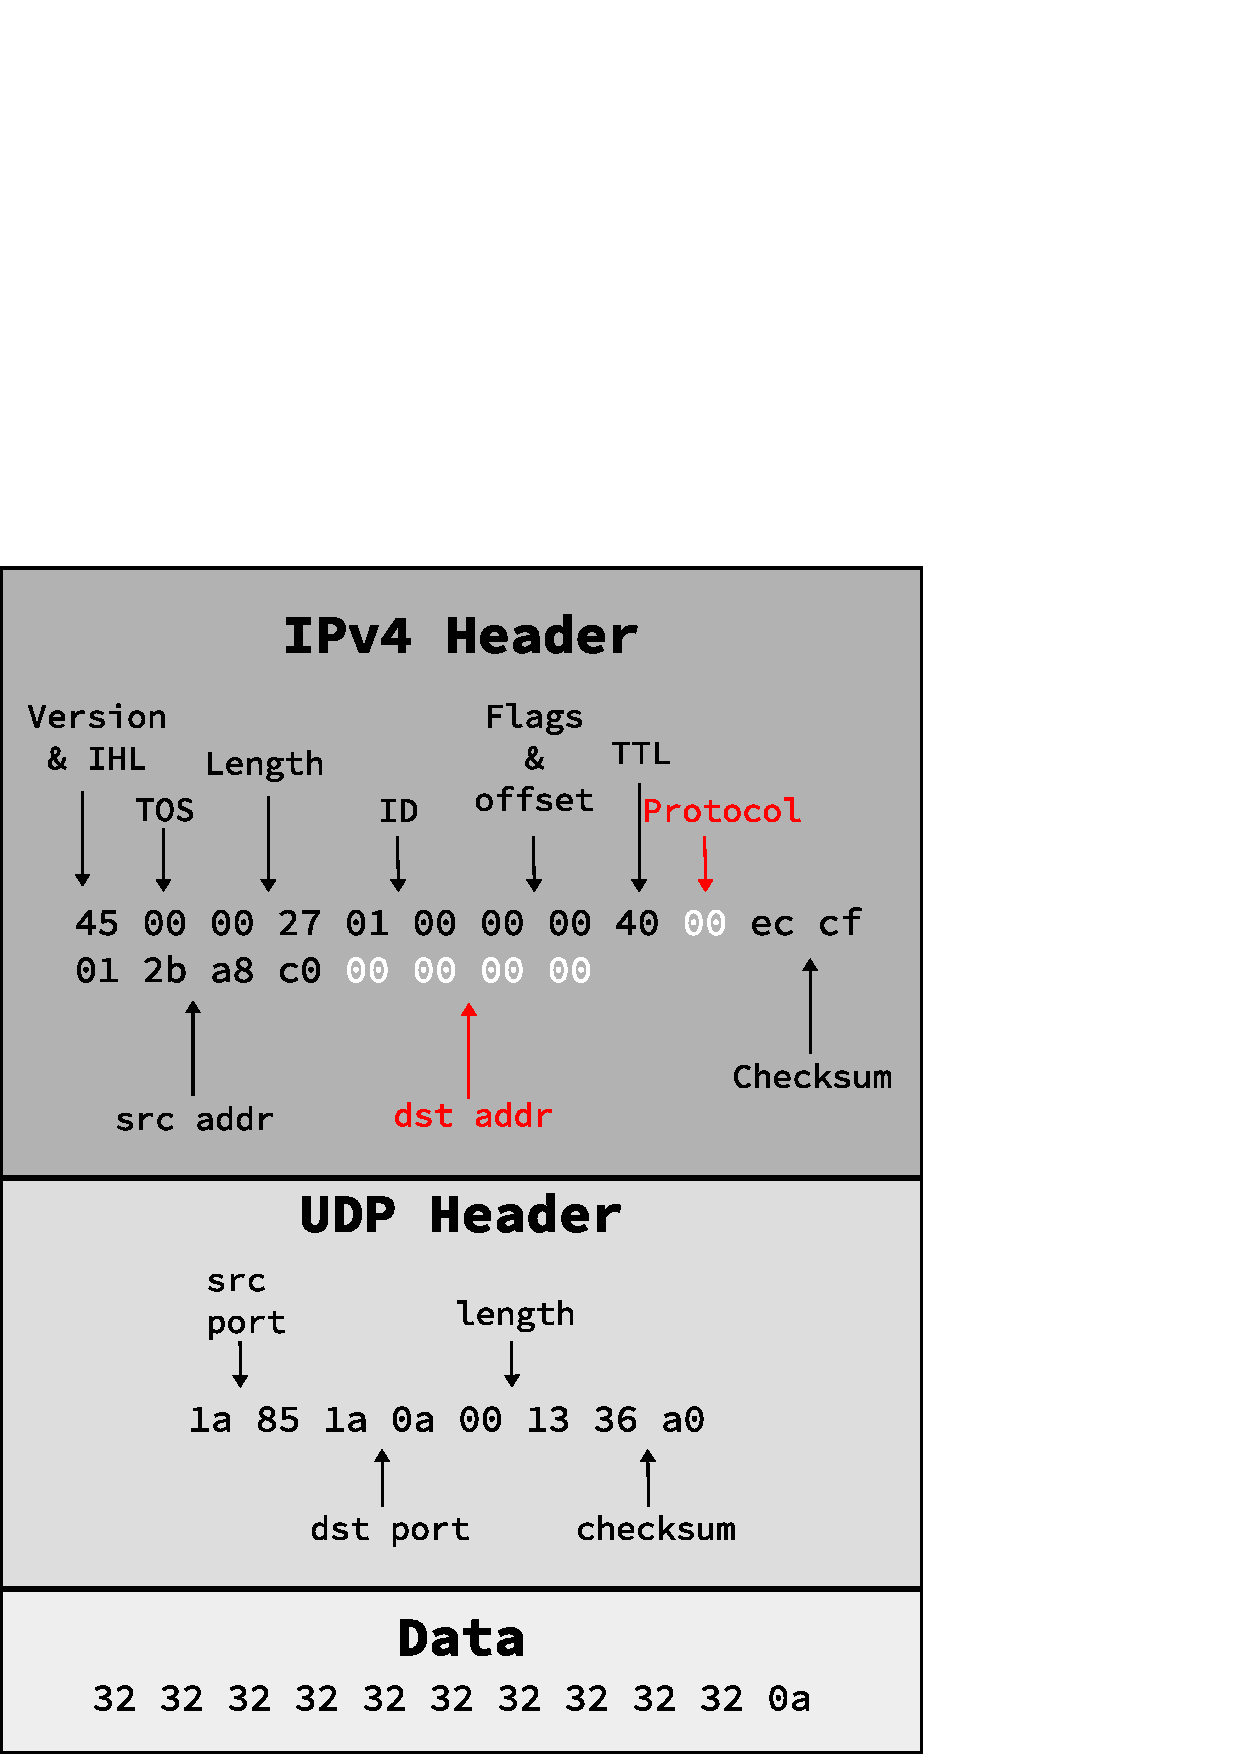
\includegraphics[width=\linewidth]{evaluation/hexdump.pdf}
	\caption{The hexadecimal representation of one of the outgoing packets
	generated by the system. Notice the red fields, indicating an error.}
\label{fig:packet_hexdump}
\end{figure}

The test has demonstrated that the packets themselves arrive at their
appropriate destinations intact. The test-suite tests all the supported
features, such as various protocols, port numbers, multiple connections through
sockets, etc.

To verify that the outgoing packets are formatted correctly, the output has
been captured and dumped into raw binary files. These can be interpreted by
numerous network utilities, such as the most well-known Wireshark.
These tools quickly detected malformations of the packets -- the
\texttt{protocol} field of the \gls{ipv4} header was not set, nor was the
destination address set. However, all offsets were calculated correctly, and
the packets had the exact proper lengths.
\autoref{fig:packet_hexdump} shows the raw binary dump of a packet, with the fields
marked.


\subsection{Internet Protocol Suite compliancy as per RFC 1122}
The networking stack was designed and implemented to comply with the networking
standards specified in RFC 1122. Although the number and size of the standards
required to be fully compliant with the Internet Protocol Suite is way over the
scope of this project, the list of requirements is a useful tool to get an
summary of the capabilities of the system.

\autoref{tab:rfc_compliance} shows a subset of the required features.
Features and protocols unrelated to this project have been removed, and can be
assumed to not be supported. The full list can be seen in \cite[Section 3.5,
Page 72]{RFC1122}.

 % Rename this to "Verification" for FPGA lingo?
\chapter{Discussion}
\label{chap:discussion}
The intent of this project was not only to implement an efficient, high-speed,
and responsive TCP/IP stack, but also to test the viability of \gls{sme} for
this types of projects. In this chapter, the results from the tests are
investigated, the viability of the networking stack is discussed, and the usage
of SME for this project is examined.

\section{Compiling to hardware}\label{sec:compiling_to_hardware}
Since the \gls{sme} \gls{vhdl} code generator never converted the project, it is hard
to comment about the codebase working on hardware.\\
However, we did notice a problem in \autoref{subsec:dictionary} regarding
the dictionary implementation. To find a value in the value table, it may have
to traverse the same table multiple times in random order. This means that the
value list would be iterated over at most $n$ times. In each iteration there are
$n$ branches. The total amount of branches for the operation is therefore $n^2$.
In the current design, this happens in one clock. This would result in a very
long path with multiple lookups, multiplexers and number operations in one clock.
This is far from ideal, and would possibly prevent the system to be implemented
on average hardware.\\
A possible solution is discussed in \autoref{subsec:bug_dictionary_lookup}


\section{Performance}
In the test chapter \ref{chap:evaluation}, we ran the simulation for
multiple hours. In about 2 million clock cycles, the networking stack was able
to handle 17283 packets in total, where 1280 of the packets were valid
connections intended for the user of the stack. During the test, the valid
data-stream was also sent out in identical 1280 packets.\\ % \notemark{Fix!}
If the network stack was clocked at a very modest clock-rate of 10 MHz of the
maximum 866 MHz on the Xilinx Zynq-7000 series\cite{xilinx_zynq_7000}, the
network is theoretically able to run at:
$$1\:\mathbf{Byte}*10\:\mathbf{MHz}= 80\:\mathbf{Mbps}$$

This speed is by no means exceptional, in fact, it is very slow compared
to even common ethernet network adapters found in consumer server hardware, such
as the Intel Ethernet I210 series\cite{intel_1gbps_nic}.\\

However, the network stack never reached the actual hardware, so the
theoretical speed is questionable. Furthermore, since the most resource-heavy
processes cannot be investigated, optimization of the stack would be premature
as of now.


% 118400 packets in total
% 1280 ingoing
% 1280 sent
% clocks: 10 000 000 mio.


\subsection{Improving performance}


\begin{figure}
\centering
\includegraphics[width=\linewidth]{discussion/design_stacked.eps}
\caption{Replicating the "inner" part of the design in order to multiply the
performance. }
\label{fig:design_stacked}
\end{figure}


Even though many optimizations can be done on the network stack codebase
itself, there are other ways of achieving better performance from the project.

\subsection{Increasing the throughput by widening the data channel in the
busses}
Perhaps the most instinctual way of improving the performance of a network
stack is by increasing the throughput. By increasing the width of the
\texttt{data} channel in the buses carrying information, the throughput could
potentially increase manyfold.

While this change is perfectly doable in the hardware and easy to implement in
the code, it might also have some unexpected consequences on the logic of the
processing modules.

For example, while not strictly a requirement, most, if not all, header sizes
are a multiple of 8 bits. By transferring only 1 byte at a time, the system is
sure to never cross the boundary of a header in the same clock cycle. If,
however, the data-bus transferred 2 bytes at a time, the first byte might be
the last part of a header, while the next byte is a data-byte. In that case,
the process has to not only parse the finished header, but also forward the
second byte down to the next process. Here again will the processes need
additional logic needs to check how much of the data-bus actually contains
valid data. Figure \ref{fig:bus_width_boundaries} illustrates the problem of a
data-segment not aligning with the bus-width.

\begin{figure}
\centering
\includegraphics[width=\linewidth]{discussion/bus_width_boundaries.eps}
\caption{Misaligned data in an extended data-bus. }
\label{fig:bus_width_boundaries}
\end{figure}





\subsection{Replicating the system}
During the design-phase, it was important to ensure the active connections
arrived on the same stack, since the IP fragments have to be collected on the
same buffer, and the TCP state has to be synchronized.

The \texttt{Transport} is especially burdensome, as it has to handle both
ingoing- and outgoing-packets, as well as the user interface calls and
protocol-specific handshakes and other operations. Finding a way of getting
around this congestion, it should be possible to parallelize the system for
better performance.

By replicating the networking stack and assign a unique IP address to each, it
should be possible to create a "Load Distributor", distributing the packets
across multiple networking stacks. Figure \ref{fig:design_stacked} shows a
prototype design, where the inner part of the networking stack is duplicated on
the FPGA itself. The \texttt{Load Distributor} conveys the packets to the
appropriate network-stack.

On the other side of the same figure, the \texttt{Load Collector} ensures that
the replicated network stacks work as one, and that they are abstracted away
in the \texttt{User Interface}, so that the user does not have to make up for
the separation. Even though the \texttt{Transport} processes do not share any
information across the stacks, they can have hardcoded \texttt{socket} numbers,
assigning a block of sockets to each stack, so that overlap does not happen.


\section{Usability}
Perhaps the most important aspects of any software project is its usability,
versatility, and its application.
While it is shown in chapter \ref{chap:evaluation} that the networking stack
performs arguably well in a reasonable simulated scenario, it is to be seen
whether the project can bring any value to the user.

\subsection{Intended usage}
The intended usage of the networking stack is to be integrated with existing
FPGA hardware in order add networking capability to a system. These systems
range from simple embedded \gls{iot} devices to large \gls{nic} cards.\\
Although it is possible to connect an SME project with other VHDL projects, it
is much more straight-forward to add the networking code directly into an SME
project.\\
For instance, other SME projects, such as the "High Throughput Image Processing in X-ray
Imaging" developed by Troels Skjøttgaard Ynddal\cite{troels}, which does
real-time image processing on x-ray images, could benefit from a network stack
by sending the processed images to a server for further analysis and backup.

\subsection{Existing solutions}
Sadly, the developed networking stack could not be brought onto an \gls{fpga},
making the comparison to existing solutions difficult.
In theory, if the networking stack worked on an FPGA, it would bring little to
no runtime advantages over existing FPGA TCP/IP stacks, such as the
Xilinx 10Gbps TCP/IP Stack\cite{sidler2016lowlatencytcp}.
However, the networking stack is easily extensible and modular. The design
choices made during the development have proven to make the stack very flexible,
and the programmer can easily add or remove protocols. The use of the C\#
programming language makes it more accessible for software engineers to modify
the code without prior knowledge to the hardware itself, or special \gls{hls}
tools and languages, albeit without the dynamic constructs of the C\# language.


\subsection{Integration with existing hardware}
As an extension to this project, the code for the Digilent Pmod NIC100\cite{pmod_nic100}
has been developed by Carl-Johannes Johnsen to act as the \texttt{Link Interface}
\cite{carl_pmod_nic100}, so that the networking stack could be tested on real
hardware.
While the stack never reached bare-metal, the testing suite simulates this
connection from the Pmod100 into this \texttt{Link Interface}. Although testing
on real hardware has to be carried out for definitive results, the simulation
suggests that this connection with networking hardware can indeed work.


\section{Using C\# with SME}
Not only had the use of C\# with \gls{sme} a great impact on the design, but the
whole project as a whole.

\subsection{Concurrency}
As was the intent of the \gls{sme} project, the messaging framework was
indispensable during the development of the networking stack. Besides not
having to concerns ourselves with the synchronization across processes, the
"Shared Nothing" property of \gls{sme} was a great help during the design, and
forced the design to be neatly isolated in the appropriate layers.

The isolation of each \texttt{Process} object gave a great overview of what each
"thread" of the system was doing. Likewise, the information exchange was very
clear, since it was nicely collected in one place -- the bus.

Sadly, the parsing of network packets is excessively sequential, and the
project does not utilize the full potential of SME in that regard.

\subsection{Cumbersome initialization and alternation}
% Parallelism hard from software
% Initialization of busses is cumbersome
The way projects are written in SME with C\#, the programmer has to
choose a design hardware architecture beforehand, since adding new SME
processes after the fact is cumbersome, and requires a lot of manual
modifications.
For instance, injecting a new process in between two existing processes
requires potentially adding new busses to the system and set these up correctly
in the code. Although this is a trivial task, the process itself is prone to
typos and oversights from the programmer.


\subsection{Using the C\# language}
In the beginning, it was pleasant to use a familiar language for the
implementation of the networking stack. Yet, as the code-base grew in size, the
flaws started to surface.

The C\# programming language is a very actively developed language with many
modern features, it is widely used with a very active community, and it has a lot
of useful packages and frameworks.

When writing code for the simulation, all of these utilities and features can
be used, providing the programmer with endless possibilities for
simulation-scenarios. For instance, in this system, the simulation processes use the
file-system to load pre-recorded packets and feed them into the
simulation or to create log-files of the simulation\footnote{
A number of experiments have also been carried out in order to replace the
native networking stack with the simulation}.

Unfortunately, almost none of these features are available with \gls{sme}
when writing code for the FPGA, as most of these require dynamic constructs,
such as instantiation of new classes or use of dynamic collections. Although
this restriction is caused by the hardware and not \gls{sme} itself,
the C\# language started to be much less intuitive. Instead of applying
best practices and exploring new features in a well-known and established
language, we had to limit ourselves to the viable subset of the working
features, and create the design around it. While it is understandable why
a proven language is used to test out a new message passing framework,
the C\# language did not always feel right for hardware development, and
the upcoming \gls{smeil} might prove itself to be a welcome addition to
the \gls{sme} project.\cite{github_smeil}.


\subsubsection{Pre-written components and modules}
The \gls{sme} framework already contains premade objects for use, such as the
\texttt{TrueDualPortMemory}, which is a process that helps the programmer write
code interfacing with the built-in block memory on the \gls{fpga}.\\
As of yet, only a few memory components are included in the \gls{sme}
framework.

During development, there was a pattern of prevailing components and systems
reused in multiple processes:
\begin{itemize}
\item \textbf{Generic buffer process}\\
As documented in the design section, the buffers make up a big part of
functionality in the whole system. However, these \gls{fifo} constructs
are very commonly used during FPGA development\cite{fpga_fifo}. A generic
\gls{fifo} buffer component would be a very useful feature during the
development of the networking stack.

\item \textbf{AXI4 communication process}\\
In the processes, the programmer is free to implement any bus interface signal
protocol. Although a custom protocol was implemented for the system, it has
been cumbersome and challenging to implement two processes with a shared signal
protocol. Pre-written processes with support for established signal protocols
could be a valuable addition to the \gls{sme} ecosystem.

\end{itemize}


\subsection{Process state modelling}
Most processes in the system have multiple states, some containing fairly
complex state-transitions, as seen on figure \ref{fig:statemachines_internetin_transport}
in chapter \ref{chap:implementation}.\\
Introduced in the implementation chapter, \gls{sme} provides the
\texttt{StateProcess} class to simplify the creation of processes with
multiple states. This class proved itself to be immensely helpful in the
\texttt{Internet Out} process, which consist solely of sequential states.
Unfortunately, this construct is inadequate and incomplete to model the rest of
the computing processes, which were slightly more complex state-machines, as
those used in the system.

\subsubsection{Repeated code}
\begin{figure}
\centering
\includegraphics[width=\linewidth]{discussion/fsm_prestates.eps}
\caption{An example of a process state-machine with pre-checks regardless of
the current state.}
\label{fig:fsm_prestates}
\end{figure}

The first identified issue was that most processes need to run certain checks on the
start of each clock cycle, such as checking the validity of the busses,
ensuring that there were no errors in the data-stream, maintain a bus signal
protocol, or make sure that some other limitations are met.
With the conventional \texttt{StateMachine}, this is intricate to write these
checks without much repetition. Instead, in this project, regular processes are
used in combination with an internal variable keeping track of the state.
This subtle difference lets the programmer have a unified entry-point to the
code, and branching code can be written to enter the appropriate
state-functions in the code.
For instance, figure \ref{fig:fsm_prestates} visualizes that a unified
pre-checks can be run prior to enter state-specific code. This adds a lot to
the length of the "code-path", but it avoids a lot of repetition in the code.


\subsubsection{Complicated state changes}
Another common issue with modelling state-machines with \gls{sme} was certain
state-changes. In situations where a process is executing the last cycle of a
state that writes to some bus, a state-change is often desired in the end.
However, most state-transitions need to do some cleanup, for instance resetting
variables or re-initialize busses. If this cleanup happens in the same clock as
the last byte is written to the bus, this value will never arrive at the other
end. To circumvent this, the \texttt{Finish} state was utilized, which delays
the state-transition a single clock, giving the busses a clock-cycle window to
propagate correctly.

While this solution worked fine, the code itself was identical across processes
with this issue, and re-implementing was cumbersome and error-prone.

\subsection{Bugs and other lesser issues}
The\gls{sme} framework has been surprisingly stable, albeit with a few minor
bugs. Although most of these issues are being fixed at the time of writing,
they were still a noticeable hindrance during development:
\begin{itemize}
\item \textbf{Reserved VHDL keywords}\\
Certain words in the C\# code were reserved in\gls{vhdl}. While this is a
non-issue if the project is not being compiled to \gls{vhdl} code, this needed
to be taken into consideration during development. One such reserved word  was
the "Transport", used to denote the \texttt{Transport} process class.

\item \textbf{C\# structs}\\
A lot of information has to be passed between the buffers and processes. For
the sake of readability and maintainability of the codebase, this data is best
encapsulated in namespaces for a hierarchical organization.
Luckily, \texttt{struct}s became available shortly after the discovery of this
requirement, and are used in the project. For instance, the
\texttt{InterfaceBus} uses two of the \texttt{InterfaceData} struct.

\item \textbf{Slow simulation}\\
The tests carried out during the evaluation of the system were astonishingly
slow. While the simulation ran at an acceptable rate in the beginning, it
started slowing down as the test progressed. A simulation lasting multiple
hours only managed to simulate a few millions of clock-cycles.

It is important to note that this SME/C\# simulation speed can still be faster
than other VHDL simulators under certain scenarios, but it is property to
improve nonetheless.


\end{itemize}



\section{Discussion}
\begin{frame}
  \frametitle{Discussion}


\begin{columns}
\begin{column}{0.5\textwidth}
\begin{itemize}
\item<1->Performance
\item<2->Usability
\item<3->Using C\#
\end{itemize}
\end{column}

\begin{column}{0.5\textwidth}
% \includegraphics<1>[scale=0.5]{congest.eps}
\end{column}
\end{columns}





\end{frame}

\section{Conclusion}
\begin{frame}
  \frametitle{Conclusion}

\centering
Conclusion

\end{frame}




% - Network API and interfacing
% - Test setup
%   - Code tests (simulations)
%   - FPGA
%   - Real applications
% - Results and discussion
% - Conclusions
% - Future Work





\newpage
\clearpage % force new page(?)
\newpage

\onecolumn

\appendix
\begin{appendices}

\end{appendices}

\newpage
\bibliography{bib}{}
\bibliographystyle{plain}


\end{document}
